%  LaTeX support: latex@mdpi.com 
%=================================================================
\documentclass[ai,article,submit,pdftex,moreauthors]{Definitions/mdpi} 

%=================================================================
% MDPI internal commands - do not modify
\firstpage{1} 
\makeatletter 
\setcounter{page}{\@firstpage} 
\makeatother
\pubvolume{1}
\issuenum{1}
\articlenumber{0}
\pubyear{2025}
\copyrightyear{2025}
\datereceived{ } 
\daterevised{ }
\dateaccepted{ } 
\datepublished{ } 

%=================================================================
% TikZ for architecture diagram
\usetikzlibrary{arrows.meta, positioning}

%=================================================================
% Full title of the paper
\Title{Exploratory Evaluation of Class Rebalancing and GAN Augmentation for Skin-Lesion Classification}

% Author Orchid ID
\newcommand{\orcidauthorA}{0009-0006-0048-5767}

% Authors
\Author{Ogwumike Ugochukwu Belusochim Phillips $^{1,}$*\orcidA{}}

% MDPI internal command: Authors, for metadata in PDF
\AuthorNames{Ogwumike Ugochukwu Belusochim Phillips}

% Affiliations
\address{%
$^{1}$ \quad Illinois Institute of Technology, Chicago, IL, USA; bogwumike@hawk.illinoistech.edu}

% Corresponding author
\corres{Correspondence: bogwumike@hawk.illinoistech.edu}

% Abstract
\abstract{I compared class rebalancing with and without DCGAN-generated images for skin-lesion classification on HAM10000. In one train/test split, the resampling-only model reached 85\% accuracy (0.85 macro-F1) on 5,250 test images; continuing training after 3,500 synthetic images were added to the training set reduced accuracy to 80\% on 1,050 test images. A subgroup analysis based on image brightness showed the equalized-odds difference decrease from 0.13 to 0.07. Three design limitations, documented in the provenance record released with the code, prevent the 85-to-80 change from being read as the effect of synthetic augmentation. First, oversampling with replacement was applied before the train/validation/test split, so identical images recur across all three partitions and neither accuracy is measured on a held-out test set. Second, the two arms were scored on different test sets---750 versus 150 images per class---so the two accuracies are not comparable quantities. Third, the 3,500 synthetic images came from a single unconditional generator and were assigned the seven class labels by output filename, so an eighth of the 28,000 augmented training rows is label noise drawn from one distribution. The 85-to-80 change is therefore not an estimate of the effect of synthetic augmentation. HAM10000 further provides no validated skin-tone labels, and the low-brightness test subgroup contained only 12 images. These results are exploratory and do not establish improved fairness across skin tones or clinical readiness. They motivate evaluation with validated demographic labels, larger subgroups, and repeated experiments.}

% Keywords
\keyword{medical imaging; generative adversarial networks; fairness in AI; dermatology; skin lesion classification; dataset bias; clinical decision support systems; data augmentation; EfficientNet; exploratory study; negative results} 

%%%%%%%%%%%%%%%%%%%%%%%%%%%%%%%%%%%%%%%%%%
\begin{document}

%%%%%%%%%%%%%%%%%%%%%%%%%%%%%%%%%%%%%%%%%%
\section{Introduction}

Deep learning models for dermatology diagnosis achieve dermatologist-level accuracy on standardized datasets~\cite{esteva2017, haenssle2018}, yet \textit{consistently underperform on dark-skinned individuals}~\cite{adamson2018, daneshjou2022}. A substantial part of the explanation is the composition of the training data. Widely used collections such as HAM10000~\cite{tschandl2018} ship no skin-tone annotation at all, so their composition can only be estimated by proxy; the surveys that have attempted it report these datasets to be heavily weighted toward lighter skin~\cite{kinyanjui2020, wen2022}, and classifiers trained on them show lower sensitivity on darker skin. The absence of labels is itself part of the problem, and it is a constraint this paper runs into directly. The clinical consequences are severe: skin cancer in dark-skinned populations is often diagnosed at later stages with worse outcomes, partly due to biased AI tools~\cite{agbai2014}.

Collecting diverse training data faces multiple barriers: limited imaging device access in underserved regions, lower historical enrollment in clinical studies, privacy constraints, and geographic concentration of research in predominantly light-skinned populations~\cite{wen2022}. This paper reports an exploratory attempt to probe that gap with the tools available to a single investigator: class rebalancing by oversampling, and DCGAN-based synthetic augmentation trained on the small number of low-brightness images that HAM10000 contains (40 rows, 29 distinct images).

The two-stage comparison does not isolate the effect of synthetic augmentation, and this paper reports it as exploratory. The resampling-only arm reached 85\% accuracy and the synthetic-augmentation arm 80\%, but oversampling preceded the data split, the two arms were scored on different test sets, and the synthetic labels carry no class information. Each of these limitations is sufficient on its own to prevent the comparison from isolating that effect, and all three are documented in the provenance record (\texttt{docs/RESULTS\_PROVENANCE.md}) released with the code. What the paper offers is a fully documented pipeline, a null reading of synthetic augmentation under extreme data scarcity, an explicit account of the design limitations that bound it, and a deployed research demonstrator that integrates EfficientNetB0 classification, Gemini-powered patient education, and a geolocation-based clinic finder. The demonstrator is not a medical device and has not been validated for clinical use.

A note on what the reader should take from the numbers. Every quantitative claim below is tagged by provenance. Figures reproducible from the released notebook are reported as measured; figures carried over from an earlier analysis whose code was not preserved are marked as provisional at the point of use and are retained rather than deleted, so that the record of what was once claimed stays visible.

\subsection{Contributions}

This work makes the following contributions:
\begin{enumerate}[leftmargin=*, itemsep=2pt]
    \item \textbf{A documented end-to-end pipeline}: a complete, inspectable path from HAM10000 ingestion through class rebalancing, DCGAN training, EfficientNetB0 transfer learning, and deployment, with every hyperparameter traceable to the released notebook.
    \item \textbf{A negative result on synthetic augmentation under extreme data scarcity}: adding 3,500 images from a DCGAN trained on 29 distinct low-brightness images did not improve classification, and the arm that used them scored lower. The paper argues that this is not evidence about GAN augmentation in general, because the comparison was not controlled.
    \item \textbf{An explicit account of the study's methodological limits}: contamination from oversampling before the split, non-comparable test sets, synthetic labels assigned by filename, and a brightness proxy confounded with diagnosis, each identified and quantified rather than left for a reader to find.
    \item \textbf{A deployed research demonstrator}: a Streamlit system integrating classification, patient education, and clinic navigation. It is a demonstrator only: not a medical device, and not validated for clinical use.
    \item \textbf{Reproducibility}: an open-source codebase and a provenance file that states, claim by claim, which numbers the code reproduces and which it does not.
\end{enumerate}

%%%%%%%%%%%%%%%%%%%%%%%%%%%%%%%%%%%%%%%%%%
\section{Related Work}

\subsection{Deep Learning in Dermatology}

Since Esteva et al.'s landmark work demonstrating dermatologist-level skin cancer classification~\cite{esteva2017}, deep learning has advanced rapidly. EfficientNet~\cite{tan2019} emerged as a popular choice for its parameter efficiency through compound scaling. Haenssle et al.~\cite{haenssle2018} found CNNs superior to 58 dermatologists in sensitivity, yet these successes mask a critical issue: validation is primarily on light-skinned populations.

\subsection{Bias and Fairness in Medical AI}

Algorithmic bias in healthcare is a critical concern. Obermeyer et al.~\cite{obermeyer2019} found commercial healthcare algorithms exhibit significant racial bias, while Adamson and Smith~\cite{adamson2018} identified lack of dataset diversity as a fundamental cause of disparate dermatology AI performance. Daneshjou et al.~\cite{daneshjou2022} demonstrated consistent performance degradation on darker skin across dermatology AI systems. The Fitzpatrick17k dataset~\cite{groh2021} enables fairness evaluation but remains smaller than HAM10000.

Key fairness metrics~\cite{hardt2016} include: \textbf{Equalized Odds} (equal TPR and FPR across groups), \textbf{Demographic Parity} (equal positive prediction rates), and \textbf{Calibration} (equal probability that positive predictions are correct).

\subsection{Addressing Dataset Bias}

Strategies for mitigating bias include: (1) \textbf{Data collection}---direct but slow due to logistical constraints~\cite{codella2018}; (2) \textbf{Resampling}---SMOTE for tabular data~\cite{chawla2002}, oversampling with augmentation for images~\cite{wong2016}; (3) \textbf{Re-weighting}---adjusting loss weights to emphasize minority classes~\cite{cui2019}; (4) \textbf{Domain adaptation}---aligning feature distributions across domains~\cite{ganin2016}.

\subsection{Generative Adversarial Networks in Medical Imaging}

GANs~\cite{goodfellow2014} have enabled medical image synthesis for CT-to-MRI translation~\cite{wolterink2017}, stain normalization~\cite{shaban2019}, rare condition augmentation~\cite{frid2018}, and super-resolution~\cite{mahapatra2019}. DCGAN~\cite{radford2015} introduced convolutional layers for stable training, while CycleGAN~\cite{zhu2017} enables unpaired image translation---essential for skin-tone translation since paired lesion images across skin tones don't exist. Recent work explores StyleGAN~\cite{karras2019} and diffusion models~\cite{ho2020} for higher quality but requiring more data and computation.

Fairness-aware augmentation has targeted bias mitigation: Glocker et al.~\cite{glocker2023} use balanced sampling for chest X-ray fairness, while Puyol-Antón et al.~\cite{puyol2021} employ adversarial training for demographic-invariant cardiac MRI representations. Few-shot approaches (prototypical networks~\cite{snell2017}, MAML~\cite{finn2017}) offer alternatives with $<$50 samples per class. We select DCGAN for its efficiency and comparatively modest data requirements. Our own run does not establish a sample-size threshold for it; it only shows that a generator fitted to 29 distinct images did not yield usable augmentation in this pipeline.

\subsection{Clinical Decision Support Systems}

Effective CDSS must provide interpretable outputs, workflow integration, uncertainty quantification, and patient-facing explanations~\cite{sutton2020}. Recent LLM advances enable sophisticated medical chatbots achieving physician-level performance on medical Q\&A~\cite{singhal2023}, though careful prompt engineering and safety guardrails remain essential.

%%%%%%%%%%%%%%%%%%%%%%%%%%%%%%%%%%%%%%%%%%
\section{Dataset}

\subsection{HAM10000 Overview}

We utilize the HAM10000 dataset~\cite{tschandl2018}, a publicly available collection of 10,015 dermoscopic images acquired using different modalities (dermoscopy and VivaScope). The dataset spans seven diagnostic classes with significant class imbalance (Table~\ref{tab:dataset}).

\begin{table}[H]
\caption{HAM10000 Class Distribution and Clinical Significance.\label{tab:dataset}}
\begin{tabularx}{\textwidth}{llCC}
\toprule
\textbf{Class} & \textbf{Full Name} & \textbf{Count} & \textbf{\%} \\
\midrule
nv & Melanocytic nevi & 6,705 & 66.95 \\
mel & Melanoma & 1,113 & 11.11 \\
bkl & Benign keratosis & 1,099 & 10.97 \\
bcc & Basal cell carcinoma & 514 & 5.13 \\
akiec & Actinic keratosis & 327 & 3.27 \\
vasc & Vascular lesions & 142 & 1.42 \\
df & Dermatofibroma & 115 & 1.15 \\
\midrule
& \textbf{Total} & \textbf{10,015} & \textbf{100.00} \\
\bottomrule
\end{tabularx}
\end{table}

The class imbalance ratio (majority to minority) is 58:1, presenting significant challenges for classifier training. HAM10000 ships no Fitzpatrick or other skin-tone labels of any kind, and no validated proxy for them. Prior work reports that the collection is drawn predominantly from lighter-skinned populations~\cite{kinyanjui2020, wen2022}, but this paper cannot verify any skin-tone composition figure from the data it uses, and therefore reports none. The dataset also contains multiple images per \texttt{lesion\_id}, which has consequences for splitting that Section~\ref{sec:limitations} returns to.

\subsection{Clinical Context}

Classes range from life-threatening (melanoma: 99\% to 27\% five-year survival from localized to metastatic~\cite{siegel2023}) to benign (melanocytic nevi, benign keratosis, dermatofibroma, vascular lesions). Basal cell carcinoma is most common but rarely metastasizes. Actinic keratosis is pre-cancerous (10\% progress to squamous cell carcinoma if untreated).

\subsection{Data Preprocessing}

Preprocessing is deliberately minimal, and this subsection describes only what the code does. For the classifier, each image is decoded, resized to $224 \times 224$, cast to float, and passed through Keras' \texttt{efficientnet.preprocess\_input}; no other normalisation is applied. For the GAN, images are resized to $64 \times 64$, converted to RGB, and scaled to $[-1,1]$. No hair-removal step (DullRazor~\cite{lee1997} or otherwise), no histogram equalisation, no colour normalisation, and no rotation, flip, brightness or zoom augmentation is applied anywhere in the exploratory pipeline. The controlled pipeline released with this paper applies light geometric augmentation to the training split only, and records it.

The rows are oversampled with replacement to 5,000 per class (seed 42), giving a pool of 35,000 rows, and that pool is then split 70/15/15 with stratification on the class label: 24,500 training, 5,250 validation, 5,250 test. The order of those two operations places duplicates of the same image on both sides of the split, and Section~\ref{sec:limitations} treats it as the paper's principal threat to validity.

\begin{figure}[H]
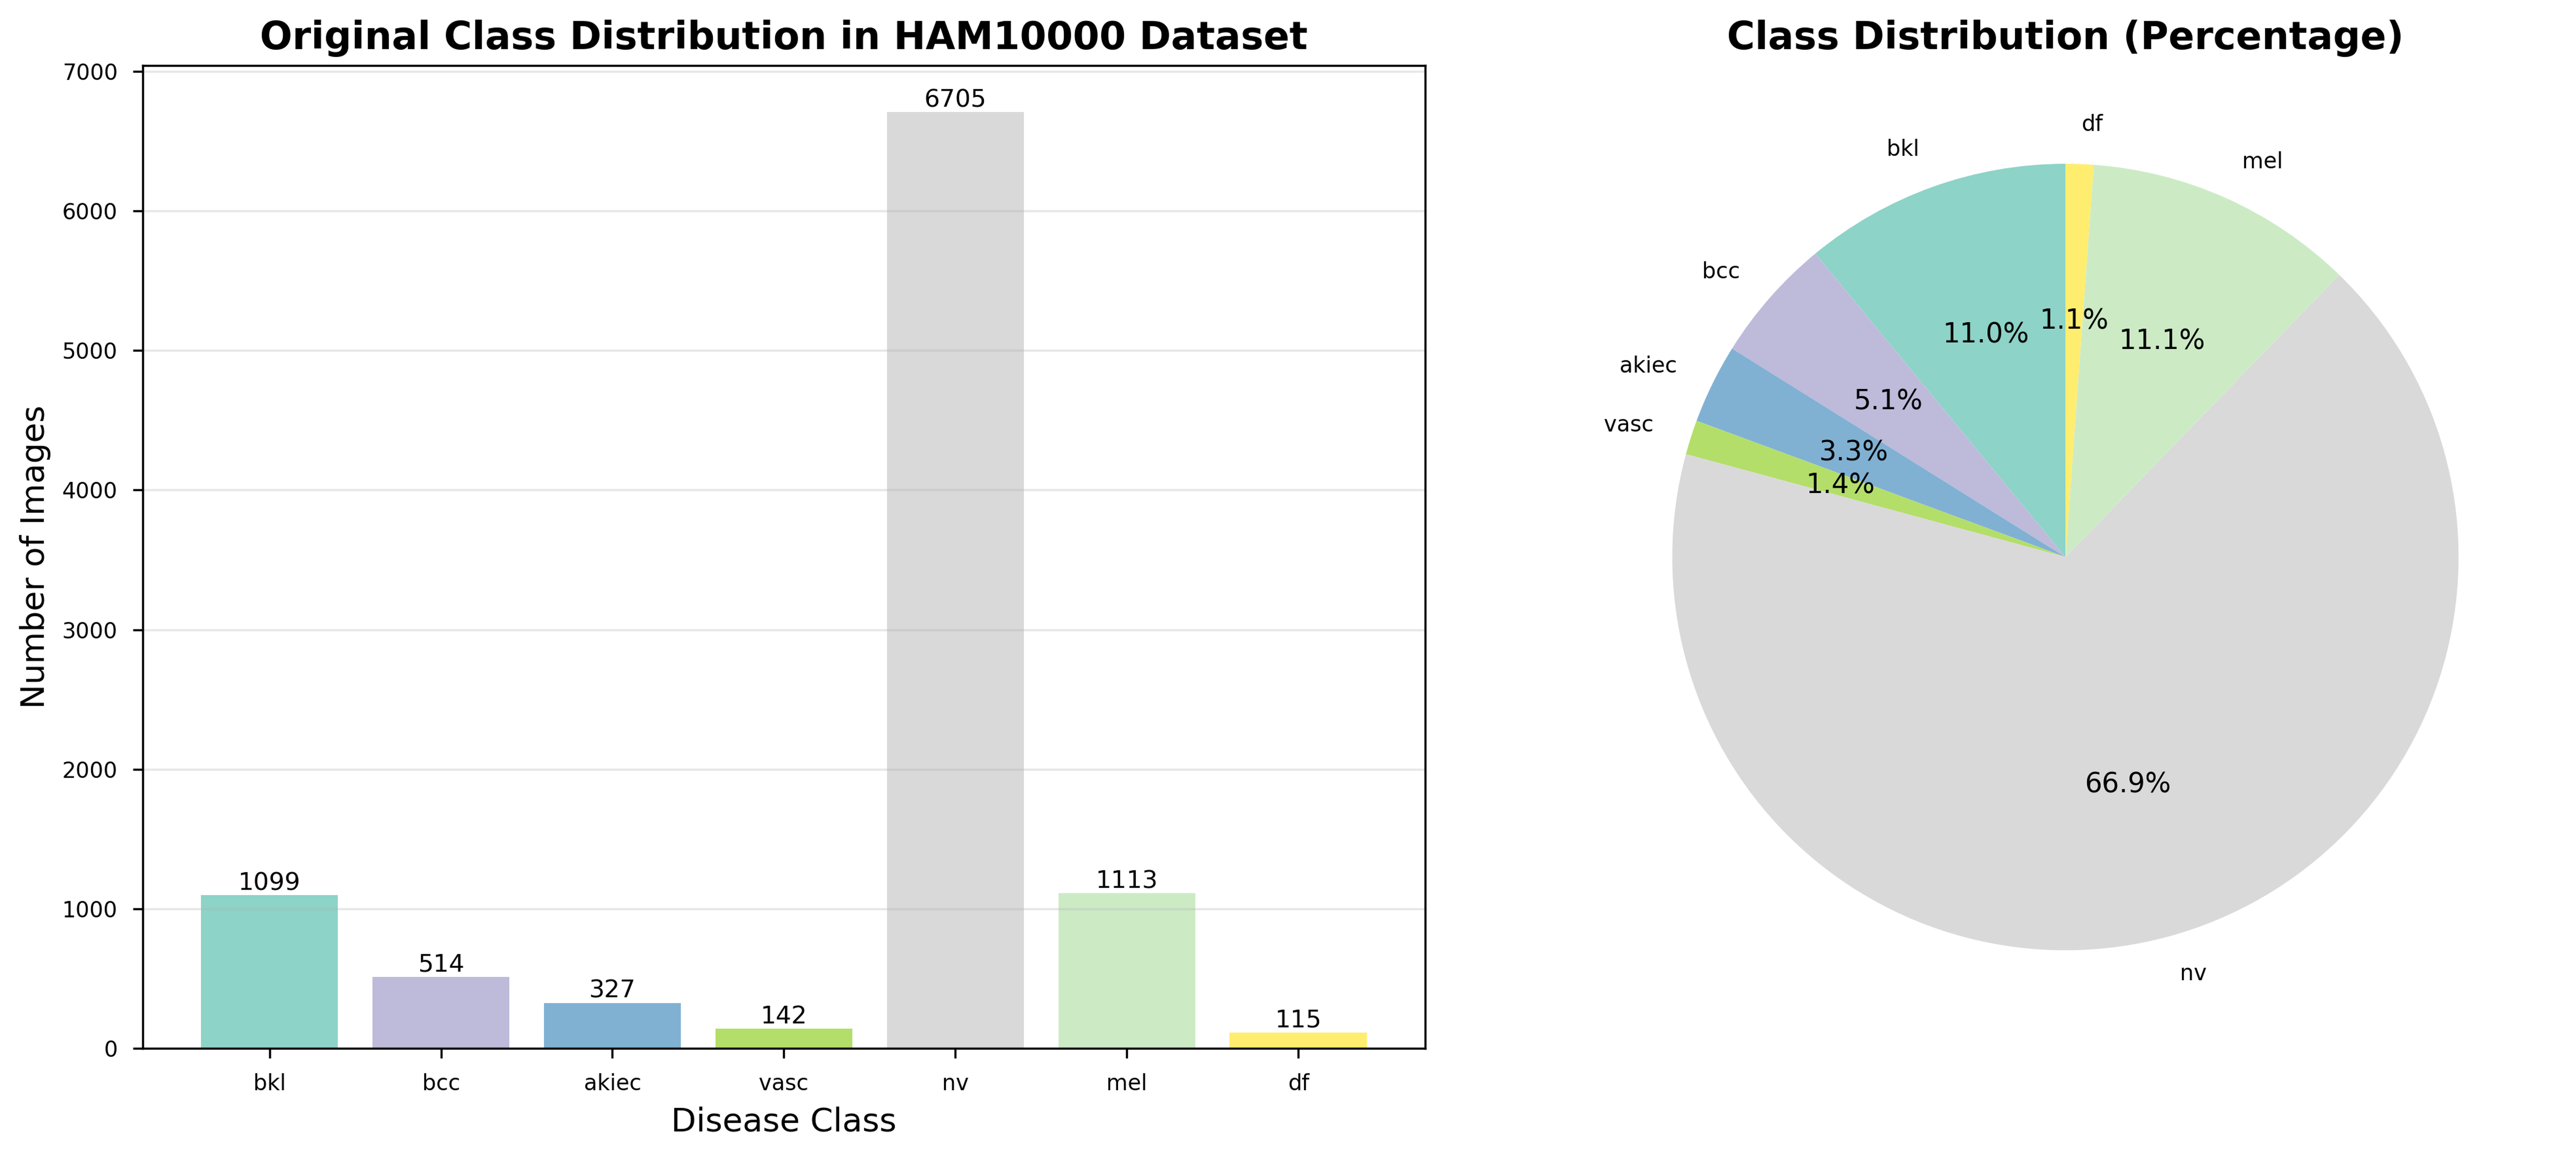
\includegraphics[width=\textwidth]{class_distribution.png}
\caption{Class distribution in the HAM10000 dataset demonstrating severe class imbalance across seven dermatological conditions. Melanocytic nevi (nv, benign moles) dominate with 6,705 samples (67\% of dataset), while rare conditions like dermatofibroma (df, 115 samples, 1.15\%) and vascular lesions (vasc, 142 samples, 1.42\%) are severely underrepresented. The majority-to-minority class ratio of 58:1 presents significant challenges for classifier training and motivates our strategic resampling approach to 5,000 samples per class.\label{fig:dataset}}
\end{figure}

%%%%%%%%%%%%%%%%%%%%%%%%%%%%%%%%%%%%%%%%%%
\section{Methods}

\subsection{System Architecture Overview}

Our system comprises four integrated modules (Figure~\ref{fig:architecture}):
\begin{enumerate}[leftmargin=*, itemsep=2pt]
    \item \textbf{DCGAN Module}: Generates synthetic dark-skin images
    \item \textbf{Classification Module}: EfficientNetB0-based diagnosis
    \item \textbf{Chatbot Module}: Gemini-powered patient education
    \item \textbf{Locator Module}: Geolocation-based hospital finder
\end{enumerate}

\begin{figure}[H]
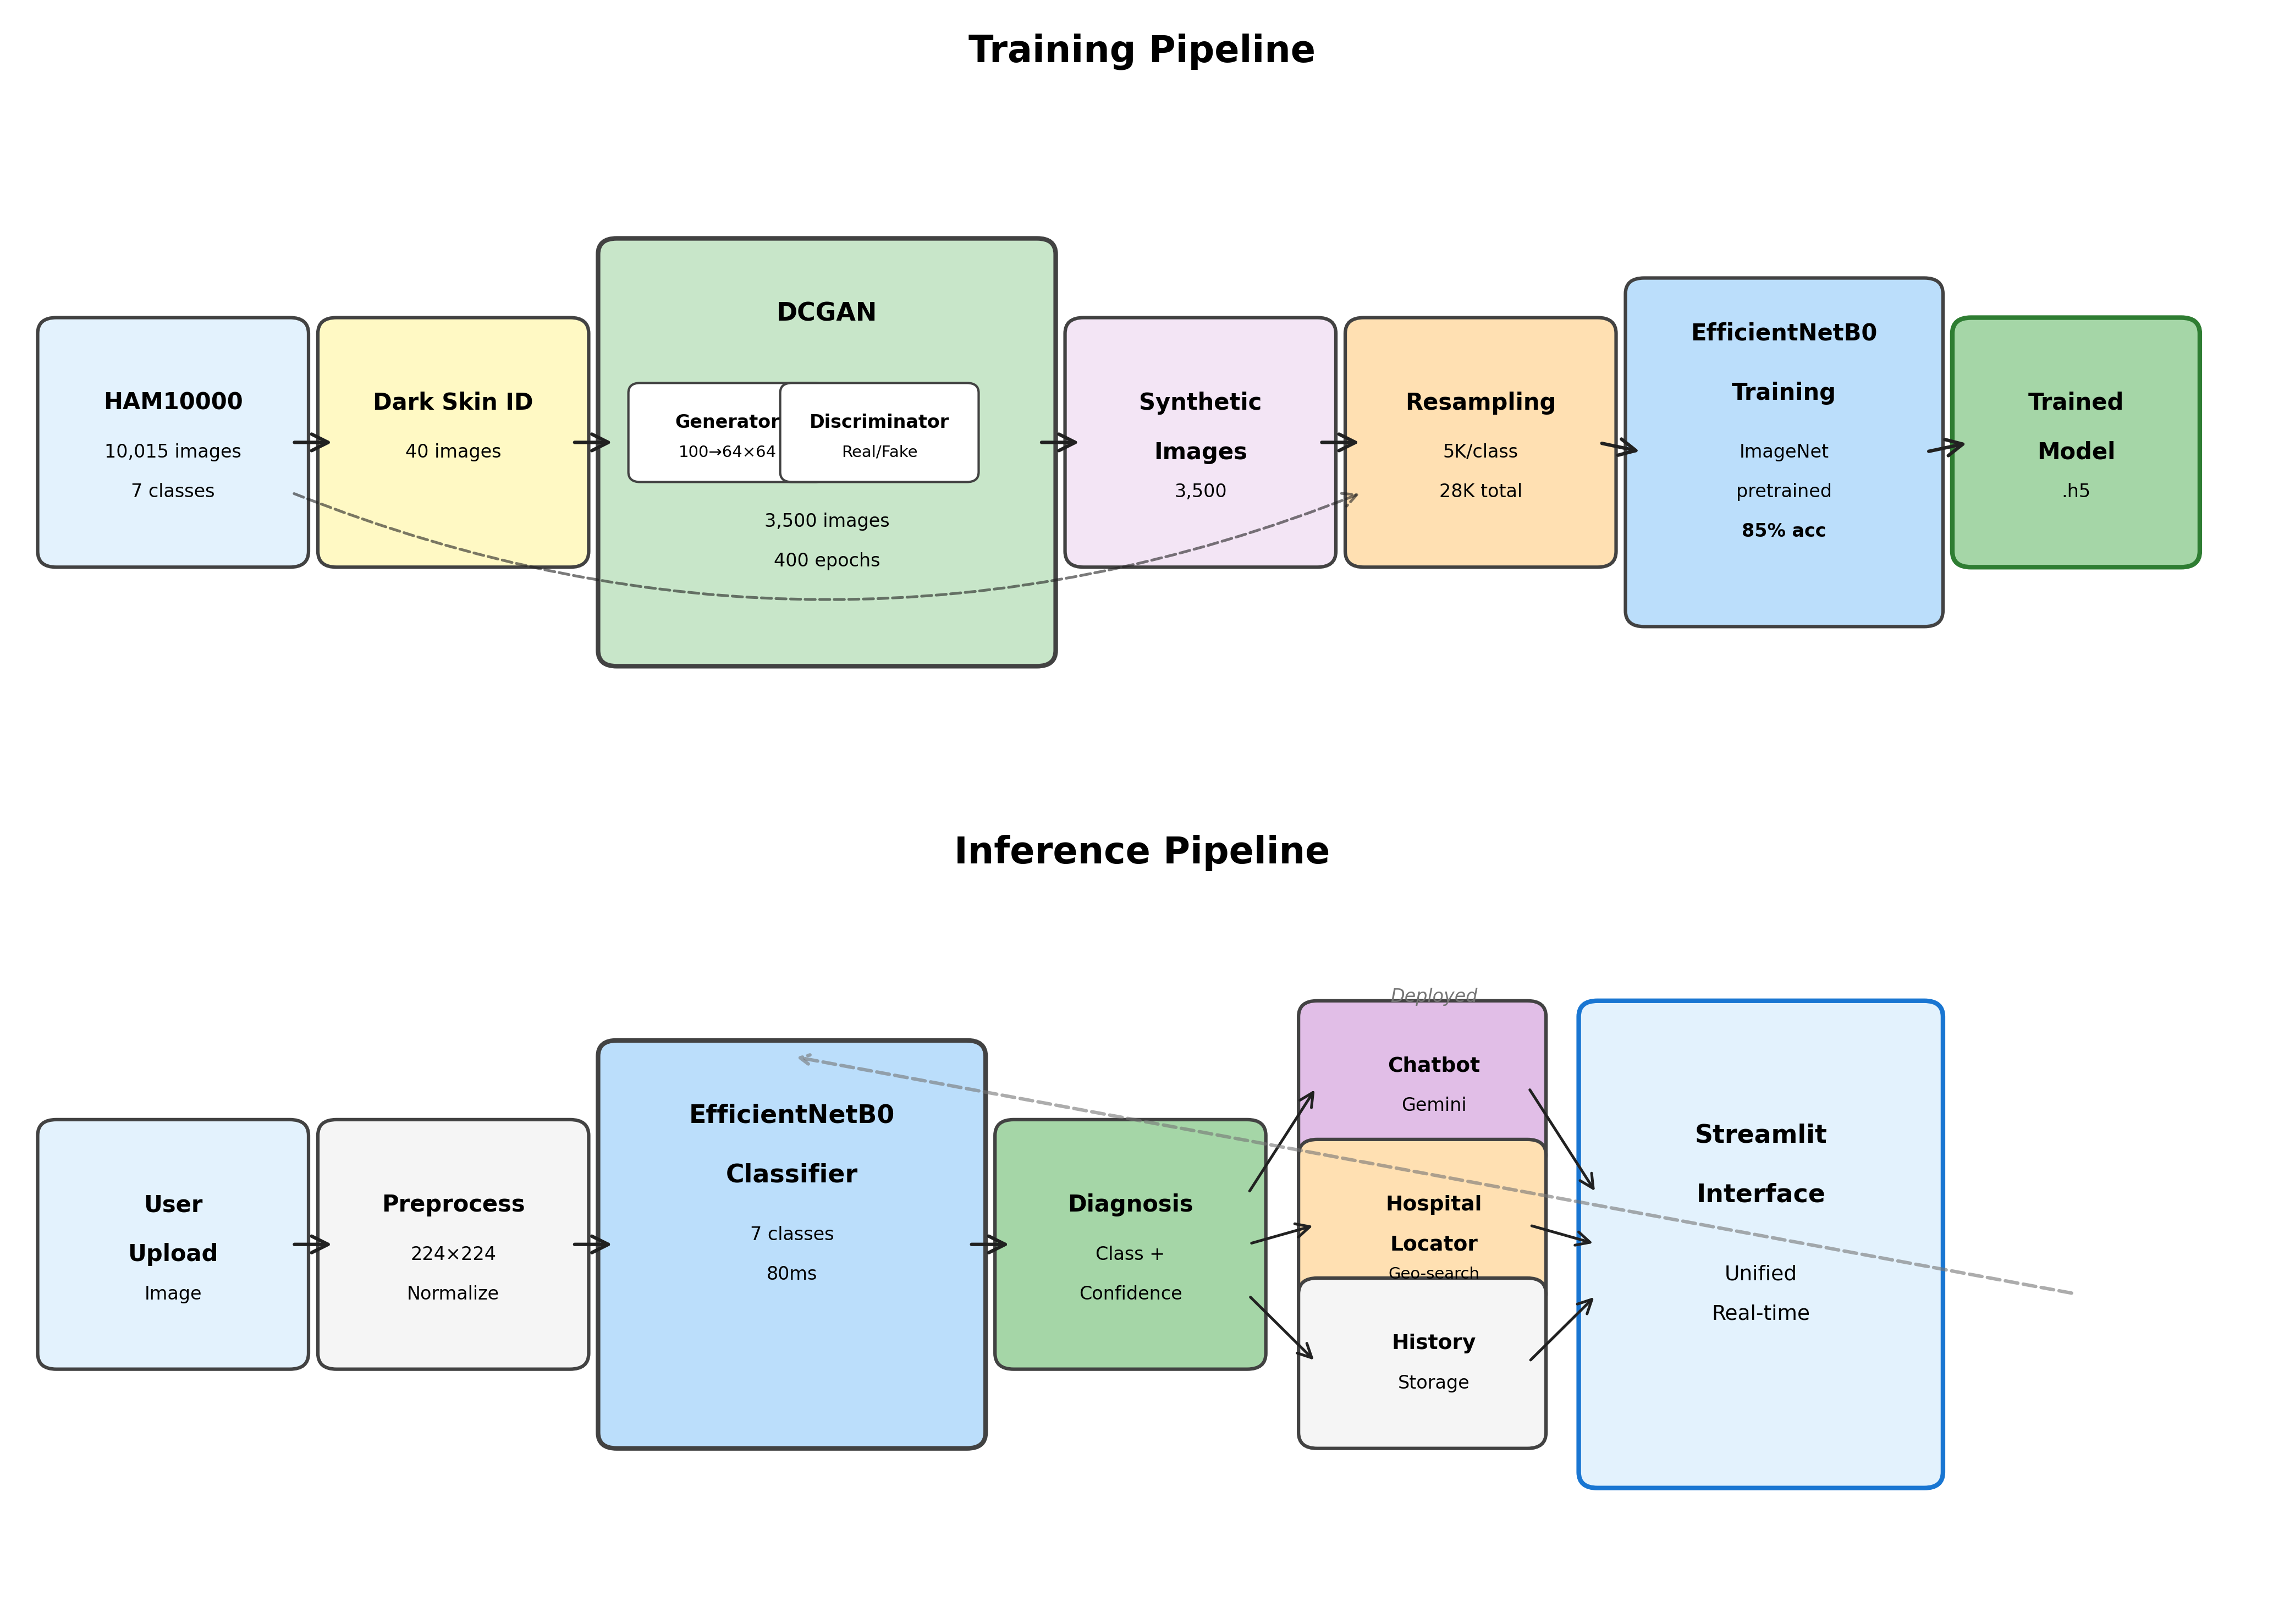
\includegraphics[width=\textwidth]{system_architecture.png}
\caption{End-to-end system architecture showing the complete pipeline from data preprocessing to deployment. The training pipeline (top) adds DCGAN-generated images to the oversampled HAM10000 training split before continuing training of the EfficientNetB0 classification head. The inference pipeline (bottom) integrates three components: (1) lesion classification with softmax confidences, (2) a Gemini-powered chatbot providing general information about the predicted condition, and (3) a geolocation-based clinic finder. The deployed artefact is a research demonstrator, not a medical device.\label{fig:architecture}}
\end{figure}

\subsection{DCGAN for Synthetic Image Generation}

A DCGAN~\cite{radford2015} was trained on the low-brightness subset, with convolutional layers in both generator and discriminator. The generator is unconditional; it takes noise and no class input.

\textbf{Generator}: Transforms 100-dimensional noise vector into 64$\times$64$\times$3 images:
\begin{itemize}[leftmargin=*, itemsep=2pt]
    \item Dense(8$\times$8$\times$256) $\rightarrow$ BatchNormalization $\rightarrow$ LeakyReLU
    \item Reshape to (8, 8, 256)
    \item Conv2DTranspose(128, 5$\times$5, stride=2) $\rightarrow$ BatchNorm $\rightarrow$ LeakyReLU $\rightarrow$ (16, 16, 128)
    \item Conv2DTranspose(64, 5$\times$5, stride=2) $\rightarrow$ BatchNorm $\rightarrow$ LeakyReLU $\rightarrow$ (32, 32, 64)
    \item Conv2DTranspose(3, 5$\times$5, stride=2, activation='tanh') $\rightarrow$ (64, 64, 3)
\end{itemize}

\textbf{Discriminator}: Classifies images as real or fake:
\begin{itemize}[leftmargin=*, itemsep=2pt]
    \item Input: (64, 64, 3)
    \item Conv2D(64, 5$\times$5, stride=2) $\rightarrow$ LeakyReLU $\rightarrow$ Dropout(0.3)
    \item Conv2D(128, 5$\times$5, stride=2) $\rightarrow$ LeakyReLU $\rightarrow$ Dropout(0.3)
    \item Flatten()
    \item Dense(1) - no activation (logits)
\end{itemize}

\subsubsection{Loss Functions}

Both networks use plain binary cross-entropy on logits, with hard targets. No label smoothing is used; the notebook passes \texttt{tf.ones\_like} and \texttt{tf.zeros\_like} directly:
\begin{itemize}[leftmargin=*, itemsep=2pt]
    \item \textbf{Generator loss}: $\mathcal{L}_G = -\mathbb{E}[\log D(G(z))]$ where $z \sim \mathcal{N}(0,1)$ and $D(G(z))$ is the discriminator's probability that generated images are real
    \item \textbf{Discriminator loss}: $\mathcal{L}_D = -\mathbb{E}[\log D(x)] - \mathbb{E}[\log(1-D(G(z)))]$ where $x$ are real images and $G(z)$ are generated images
\end{itemize}

\subsubsection{Training Protocol}
\begin{itemize}[leftmargin=*, itemsep=2pt]
    \item \textbf{Training set}: the 40 rows of the oversampled pool whose mean grey intensity is below 110. These 40 rows contain 29 distinct images; one image appears four times. The input tensor is therefore of shape $(40, 64, 64, 3)$ but spans 29 unique lesions
    \item \textbf{Optimizer}: Adam at learning rate $1 \times 10^{-4}$ for both generator and discriminator, with Keras' default momentum parameters
    \item \textbf{Training epochs}: 400
    \item \textbf{Batch size}: 32
    \item \textbf{Noise dimension}: 100
    \item \textbf{Image size}: 64$\times$64 pixels throughout. Generated images are written to disk at 64$\times$64 and resized to 224$\times$224 by the classifier's input pipeline. No GAN stage operates at a higher resolution
    \item \textbf{Conditioning}: none. One unconditional generator was trained on all 40 rows together. The seven class labels were attached afterwards, by writing 500 outputs per class to filenames of the form \texttt{class\_<k>\_img\_<i>.jpg} and parsing the label back out of the filename. The labels are therefore arbitrary with respect to image content
    \item \textbf{Hardware}: a Google Colab GPU runtime. No wall-clock training time was recorded, and none is claimed
    \item \textbf{Total synthetic images generated}: 3,500 (500 per class label $\times$ 7 labels)
\end{itemize}

% DCGAN Architecture Diagram
% Using pre-generated image for faster compilation (TikZ version available in comments below)
\begin{figure}[H]
\centering
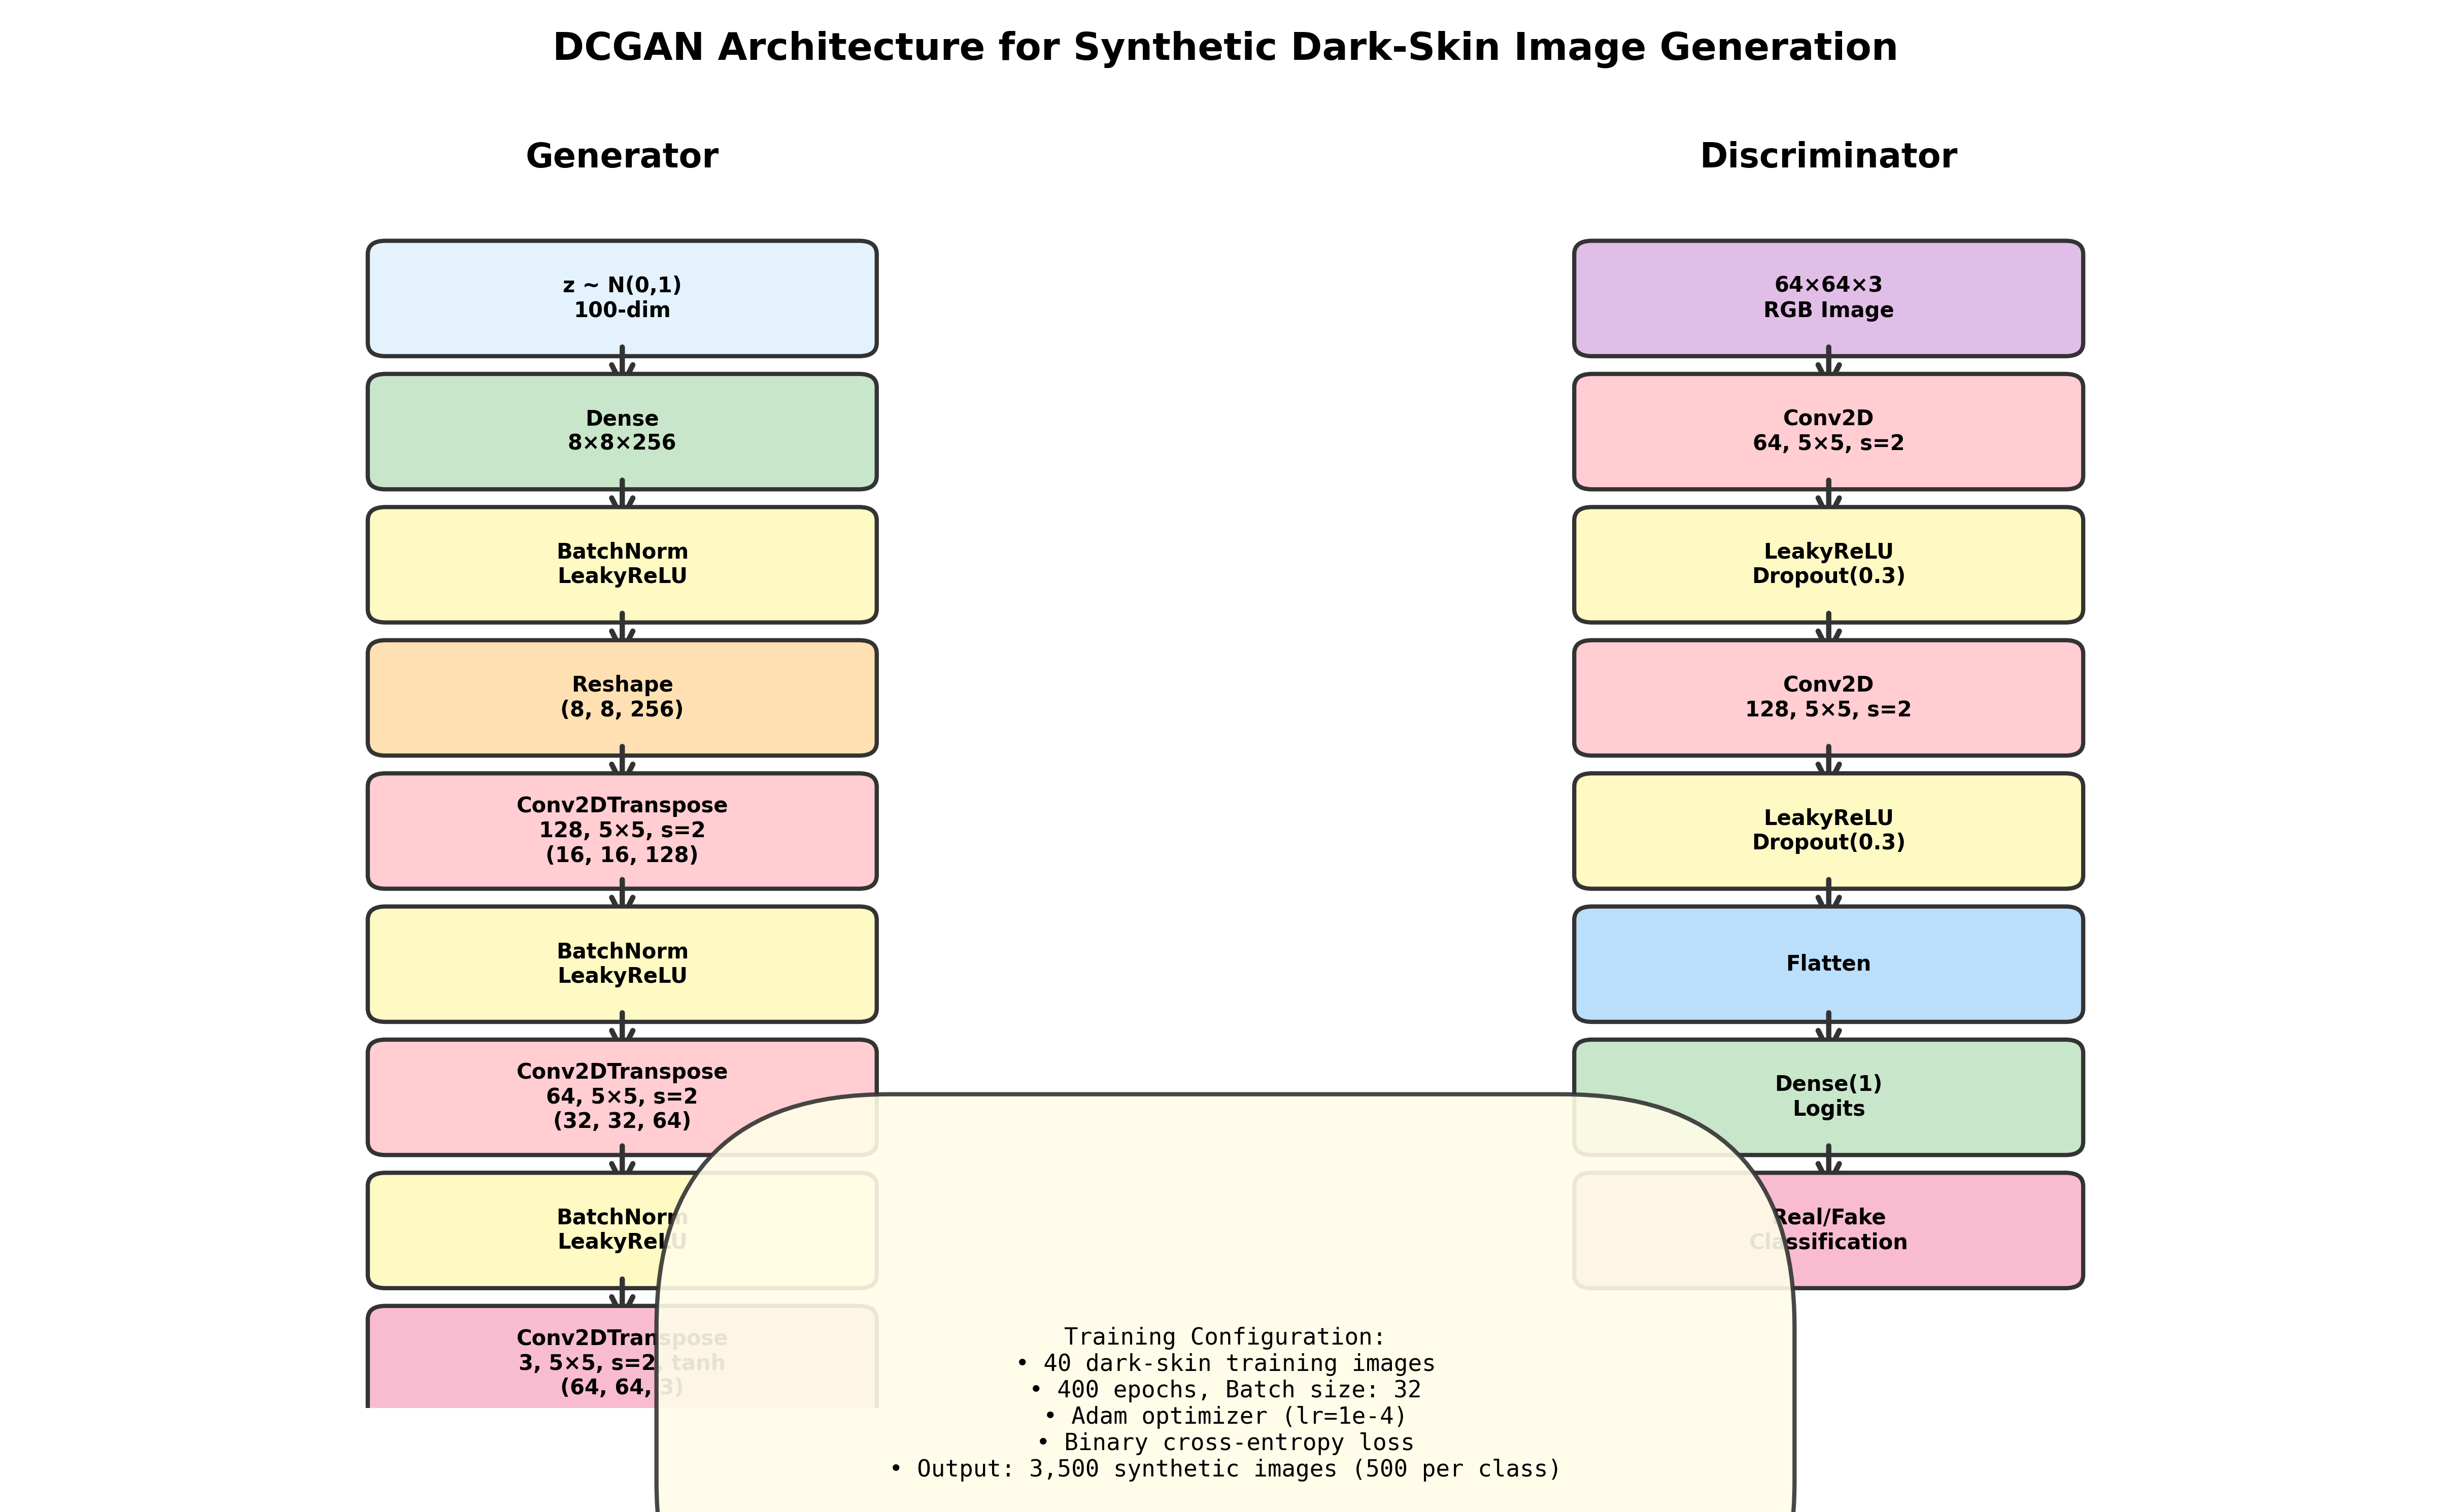
\includegraphics[width=\textwidth]{gan_architecture.png}
\caption{DCGAN architecture, as implemented. \textbf{Left (Generator):} upsamples 100-dim noise to $64\times64\times3$ RGB via transposed convolutions with BatchNorm and LeakyReLU. \textbf{Right (Discriminator):} classifies $64\times64\times3$ images as real or fake using strided convolutions, dropout, and a final dense logit. Both are trained adversarially with binary cross-entropy on logits. The generator is unconditional: it has no class input, which is why the class labels later attached to its output carry no information.\label{fig:gan}}
\end{figure}

% TikZ version (commented out for faster compilation - uncomment if needed)
% \begin{figure}[H]
% \centering
% \begin{tikzpicture}[
%     node distance=8mm,
%     box/.style={draw, rounded corners, thick, minimum width=35mm, minimum height=10mm, align=center, fill=#1},
%     arrow/.style={-Latex, thick},
%     font=\sffamily\small
% ]
% % Generator (left column)
% \node[box=blue!10] (g0) { $z \sim \mathcal{N}(0,1)$\\100-dim };
% \node[box=green!10, below=of g0] (g1) { Dense\\$8\times 8\times 256$ };
% \node[box=yellow!10, below=of g1] (g2) { BatchNorm\\LeakyReLU };
% \node[box=orange!10, below=of g2] (g3) { Reshape\\$(8,8,256)$ };
% \node[box=red!10, below=of g3] (g4) { Conv2DTranspose\\128, $5\times5$, $s=2$\\$(16,16,128)$ };
% \node[box=yellow!10, below=of g4] (g5) { BatchNorm\\LeakyReLU };
% \node[box=red!10, below=of g5] (g6) { Conv2DTranspose\\64, $5\times5$, $s=2$\\$(32,32,64)$ };
% \node[box=yellow!10, below=of g6] (g7) { BatchNorm\\LeakyReLU };
% \node[box=pink!10, below=of g7] (g8) { Conv2DTranspose\\3, $5\times5$, $s=2$, tanh\\$(64,64,3)$ };
% \node[box=purple!10, below=of g8] (g9) { Output\\$64\times 64 \times 3$ RGB };
% \foreach \a/\b in {g0/g1, g1/g2, g2/g3, g3/g4, g4/g5, g5/g6, g6/g7, g7/g8, g8/g9}
%   \draw[arrow] (\a) -- (\b);
% % Discriminator (right column)
% \node[box=purple!10, right=45mm of g0] (d0) { Input\\$64\times64\times3$ RGB };
% \node[box=red!10, below=of d0] (d1) { Conv2D\\64, $5\times5$, $s=2$ };
% \node[box=yellow!10, below=of d1] (d2) { LeakyReLU\\Dropout(0.3) };
% \node[box=red!10, below=of d2] (d3) { Conv2D\\128, $5\times5$, $s=2$ };
% \node[box=yellow!10, below=of d3] (d4) { LeakyReLU\\Dropout(0.3) };
% \node[box=blue!10, below=of d4] (d5) { Flatten };
% \node[box=green!10, below=of d5] (d6) { Dense(1)\\Logits };
% \node[box=pink!10, below=of d6] (d7) { Real / Fake };
% \foreach \a/\b in {d0/d1, d1/d2, d2/d3, d3/d4, d4/d5, d5/d6, d6/d7}
%   \draw[arrow] (\a) -- (\b);
% % Training info
% \node[below=12mm of g9, align=center, draw, rounded corners, thick, fill=gray!10, minimum width=90mm] (info) {%
% Training: 40 low-brightness rows (29 distinct images) \\ 
% 400 epochs, Adam (lr = \(1\times10^{-4}\), Keras defaults) \\ 
% Binary cross-entropy on logits, hard targets (no label smoothing) \\ 
% Output: 3{,}500 synthetic images (500 per class)
% };
% \end{tikzpicture}
% \caption{DCGAN architecture for generating synthetic dark-skin lesion images. \textbf{Left (Generator):} Upsamples 100-dim noise to $64\times64\times3$ RGB images via transposed convolutions with BatchNorm and LeakyReLU. \textbf{Right (Discriminator):} Classifies $64\times64\times3$ images as real or fake using strided convolutions, dropout, and a final dense logit. Both are trained adversarially with binary cross-entropy.\label{fig:gan}}
% \end{figure}

\subsection{Class Imbalance Handling}

We address the 58:1 class imbalance through a multi-stage resampling strategy:

\textbf{Stage 1 - Resampling}: All classes were resampled to 5,000 rows per class with replacement (seed 42), giving a 35,000-row pool that was then split into 24,500 training, 5,250 validation and 5,250 test rows. Because the resampling ran before the split, duplicate copies of the same image are distributed across the three partitions.

\textbf{Stage 2 - Synthetic Image Addition}: 3,500 DCGAN outputs (500 per class label) were appended to the stage-1 training split, giving 28,000 rows, and resized from 64$\times$64 to 224$\times$224 by the input pipeline. Stage 2 is not a second model: it continues training the stage-1 weights for 50 further epochs, with no early stopping. There is consequently no independently initialised ``GAN-augmented'' model to compare against the stage-1 model.

\textbf{Final Dataset Composition}:
\begin{table}[H]
\caption{Row counts at each step. ``Oversampled pool'' is the 35,000-row set produced before splitting; ``Stage-1 training'' is the 70\% of that pool used for training; ``Stage-2 training'' adds 500 synthetic rows per class label. Because oversampling preceded the split, rows in the training columns are not distinct images, and some of them also appear in the validation and test partitions.\label{tab:augmented}}
\begin{tabularx}{\textwidth}{lCCCC}
\toprule
\textbf{Class} & \textbf{Original} & \textbf{Oversampled pool} & \textbf{Stage-1 training} & \textbf{Stage-2 training} \\
\midrule
nv & 6,705 & 5,000 & 3,500 & 4,000 \\
mel & 1,113 & 5,000 & 3,500 & 4,000 \\
bkl & 1,099 & 5,000 & 3,500 & 4,000 \\
bcc & 514 & 5,000 & 3,500 & 4,000 \\
akiec & 327 & 5,000 & 3,500 & 4,000 \\
vasc & 142 & 5,000 & 3,500 & 4,000 \\
df & 115 & 5,000 & 3,500 & 4,000 \\
\midrule
\textbf{Total} & \textbf{10,015} & \textbf{35,000} & \textbf{24,500} & \textbf{28,000} \\
\bottomrule
\end{tabularx}
\end{table}

\subsection{EfficientNet Classifier}

\subsubsection{Architecture Selection}

EfficientNet~\cite{tan2019} uses compound scaling to jointly optimize network depth ($d$), width ($w$), and resolution ($r$):

\begin{linenomath}
\begin{equation}
    d = \alpha^{\phi}, \quad w = \beta^{\phi}, \quad r = \gamma^{\phi}
\end{equation}
\end{linenomath}
subject to $\alpha \cdot \beta^{2} \cdot \gamma^{2} \approx 2$, where $\phi$ is a user-specified compound coefficient.

We select EfficientNetB0 ($\phi = 0$) for its balance of accuracy and efficiency:
\begin{itemize}[leftmargin=*, itemsep=2pt]
    \item Parameters: 5.3M (vs. 25.6M for ResNet-50)
    \item FLOPs: 0.39B (vs. 4.1B for ResNet-50)
    \item ImageNet Top-1: 77.1\%
\end{itemize}

\subsubsection{Transfer Learning Strategy}

We employ transfer learning from ImageNet-pretrained weights, a standard approach for medical image classification that leverages features learned from large-scale natural image datasets:

\textbf{Training Strategy}:
\begin{itemize}[leftmargin=*, itemsep=2pt]
    \item Base model (EfficientNetB0) initialized with ImageNet-pretrained weights
    \item Base model frozen (not trainable) throughout. Only the classification head is trained: \textbf{8,967 trainable parameters of 4,058,538 total}. The model is thus a linear probe on frozen ImageNet features, not a fine-tuned network
    \item Learning rate: 0.001 (Keras Adam default), reduced by a factor of 0.5 on plateau (patience=3)
    \item Early stopping with patience = 5 on validation loss, with best weights restored
    \item Hardware: a Google Colab GPU runtime. Wall-clock training times were not recorded and are not reported
    \item Stage 2 resumes from the stage-1 weights rather than re-initialising, so the two reported accuracies come from one continuously trained model at two points in its history
\end{itemize}

\subsubsection{Classification Head}
\begin{itemize}[leftmargin=*, itemsep=2pt]
    \item Global Average Pooling 2D
    \item Dropout ($p = 0.3$)
    \item Dense (7 units, Softmax)
\end{itemize}

\subsubsection{Training Configuration}
\begin{itemize}[leftmargin=*, itemsep=2pt]
    \item \textbf{Framework}: TensorFlow 2.x / Keras
    \item \textbf{Optimizer}: Adam (initial learning rate: 0.001)
    \item \textbf{Loss}: Sparse categorical crossentropy
    \item \textbf{Batch size}: 32
    \item \textbf{Epochs}: stage 1 ran 48 epochs before early stopping (patience=5); best validation accuracy 0.8541 at epoch 46. Stage 2 ran a further 50 epochs with no early stopping
    \item \textbf{Training set}: 24,500 rows at stage 1; 28,000 rows at stage 2
    \item \textbf{Validation set}: 5,250 rows
    \item \textbf{Test set}: 5,250 rows at stage 1. The stage-2 classification report is computed over 1,050 rows (150 per class), so the two stages are not scored on the same test set
\end{itemize}

\textbf{Callbacks}:
\begin{itemize}[leftmargin=*, itemsep=2pt]
    \item EarlyStopping (monitor='val\_loss', patience=5, restore\_best\_weights=True)
    \item ReduceLROnPlateau (monitor='val\_loss', factor=0.5, patience=3, min\_lr=1e-6)
\end{itemize}

\subsection{Medical Chatbot}

The chatbot provides patient education through Google's Gemini large language model.

\subsubsection{System Design}
\begin{itemize}[leftmargin=*, itemsep=2pt]
    \item \textbf{Base Model}: Gemini Pro (Google Generative AI API)
    \item \textbf{API}: Google Generative AI SDK
    \item \textbf{Model}: \texttt{gemini-pro} for text generation
    \item \textbf{Context}: System prompt with medical disclaimers and safety guidelines
\end{itemize}

\subsubsection{System Prompt}

The chatbot operates under carefully designed constraints:
\begin{quote}
\textit{``You are a dermatology education assistant. Provide accurate, accessible information about skin conditions. Always recommend consulting a healthcare professional for diagnosis and treatment. Do not provide specific medical advice or diagnoses. If asked about emergencies, direct users to seek immediate medical attention.''}
\end{quote}

\subsubsection{Supported Query Types}
\begin{itemize}[leftmargin=*, itemsep=2pt]
    \item Symptom descriptions and explanations
    \item General treatment information
    \item Risk factors and prevention
    \item When to seek medical attention
    \item Clarification of diagnostic results
\end{itemize}

\subsection{Hospital Locator}

The locator service connects users with nearby medical facilities:
\begin{itemize}[leftmargin=*, itemsep=2pt]
    \item \textbf{Geolocation}: Browser-based or manual input
    \item \textbf{Search API}: OpenStreetMap Nominatim (geolocation-based)
    \item \textbf{Results}: 5 nearest hospitals/dermatology clinics
    \item \textbf{Information}: Name, address, distance, directions link
\end{itemize}

%%%%%%%%%%%%%%%%%%%%%%%%%%%%%%%%%%%%%%%%%%
\section{Experiments}

\subsection{Evaluation Metrics}

We evaluate performance using multiple metrics:

\textbf{Classification Metrics}:
\begin{itemize}[leftmargin=*, itemsep=2pt]
    \item \textbf{Accuracy}: Overall classification correctness, $\text{Acc} = \frac{\text{TP} + \text{TN}}{\text{TP} + \text{TN} + \text{FP} + \text{FN}}$
    \item \textbf{Macro-averaged Precision, Recall, F1}: Average across all 7 classes, treating each class equally regardless of sample size
    \item \textbf{Per-class F1-Score}: $F1 = 2 \cdot \frac{\text{Precision} \cdot \text{Recall}}{\text{Precision} + \text{Recall}}$ for each disease class
    \item \textbf{Cohen's Kappa}: Inter-rater agreement accounting for chance, $\kappa = \frac{p_o - p_e}{1 - p_e}$ where $p_o$ is observed agreement and $p_e$ is expected agreement
\end{itemize}

\textbf{Subgroup Metrics}~\cite{hardt2016}: the definitions below are the standard fairness definitions, but in this study the two groups $A$ and $B$ are defined by mean image brightness, not by skin tone, and the metrics should be read accordingly:
\begin{itemize}[leftmargin=*, itemsep=2pt]
    \item \textbf{TPR Gap}: $|\text{TPR}_{A} - \text{TPR}_{B}|$, the difference in sensitivity between the two brightness groups
    \item \textbf{FPR Gap}: $|\text{FPR}_{A} - \text{FPR}_{B}|$, the difference in specificity between them
    \item \textbf{Equalized Odds Difference}: $\max(|\text{TPR}_{A} - \text{TPR}_{B}|, |\text{FPR}_{A} - \text{FPR}_{B}|)$, lower being closer to parity between the groups as defined
\end{itemize}

\subsection{Experimental Setup}

The run that exists compares two points in the history of a single model, not three independently trained configurations:
\begin{enumerate}[leftmargin=*, itemsep=2pt]
    \item \textbf{Stage 1 (resampling only)}: class rebalancing to 5,000 rows per class by oversampling with replacement, with no synthetic images and no geometric or photometric augmentation of any kind
    \item \textbf{Stage 2 (resampling + synthetic)}: the stage-1 weights, trained for 50 further epochs on the stage-1 training split plus 3,500 DCGAN outputs
\end{enumerate}

No model was trained on the original imbalanced distribution, so this paper reports no imbalanced reference point and makes no claim about how much rebalancing contributed.

\textbf{What this design can and cannot support}: because stage 2 continues stage 1 rather than starting from the same initialisation, because the two stages were scored on test sets of different size (5,250 and 1,050 rows), and because oversampling preceded the split, the stage-1 and stage-2 accuracies are not two measurements of the same quantity under one changed factor. The design therefore supports a descriptive report of what happened in this run and supports no causal attribution to synthetic augmentation. Section~\ref{sec:limitations} states what a design that did support such an attribution would require.

\textbf{Alternative Approaches Considered}: DCGAN was chosen for its small compute and data footprint. StyleGAN2~\cite{karras2020} and diffusion models~\cite{ho2020} are reported to need substantially more data and compute than was available here. A class-conditional generator was not used, and that is the design choice this study would reverse first: without conditioning there is no mechanism by which a synthetic image acquires a meaningful label, so labelling generator output by filename cannot support a class-wise comparison. Conditioning on seven classes with 29 distinct images may not have produced usable samples either, but it would have yielded an interpretable result. No other augmentation technique was used: mixup, CutMix and conventional geometric or photometric augmentation appear nowhere in the code, and the released pipeline documents the augmentation it applies.

\textbf{Computational Environment}:
\begin{itemize}[leftmargin=*, itemsep=2pt]
    \item \textbf{Platform}: Google Colab, GPU runtime, TensorFlow/Keras as provided by that runtime. Exact library versions were not pinned at the time of the run and are not reported
    \item \textbf{Seeding}: \texttt{random\_state=42} was passed to the resampling and splitting calls. Global seeds for TensorFlow were not set, so the training runs are not bit-reproducible
    \item \textbf{Splitting}: a single stratified 70/15/15 split, taken after oversampling, with one run and no repetition over seeds
    \item \textbf{Preprocessing order}: decode $\rightarrow$ resize to $224 \times 224$ $\rightarrow$ cast to float $\rightarrow$ \texttt{efficientnet.preprocess\_input}
\end{itemize}

%%%%%%%%%%%%%%%%%%%%%%%%%%%%%%%%%%%%%%%%%%
\section{Results}
\label{sec:results}

\subsection{What the Single Run Produced}

\textbf{What was observed:} the stage-1 model reached 85\% accuracy and 0.85 macro-F1 on its 5,250-row test set; after 3,500 synthetic images were added and training continued, the stage-2 classification report gave 80\% accuracy and 0.80 macro-F1 on a 1,050-row test set. Both numbers are inflated by duplicate images shared across the split, and the two are not comparable with each other. They are reported here because they are what the run produced, not as an effect estimate.

Table~\ref{tab:results} lists the two stages. The stage-1 figure should not be read as a generalisation estimate and should not be compared with published HAM10000 accuracies, which are obtained on splits taken before any resampling. A leakage-free re-run on a lesion-level split is the minimum needed to place this model against the literature, and this paper does not have one.

\begin{table}[H]
\caption{Accuracy at the two stages of the single run, as reported by the notebook's classification reports. The two rows are scored on test sets of different size and composition and are not a controlled comparison; no difference column is given, because the difference between them is not interpretable.\label{tab:results}}
\begin{tabularx}{\textwidth}{lCCC}
\toprule
\textbf{Stage} & \textbf{Test rows} & \textbf{Accuracy} & \textbf{Macro F1} \\
\midrule
Stage 1 (resampling only) & 5,250 & 0.85 & 0.85 \\
Stage 2 (continued, + 3,500 synthetic) & 1,050 & 0.80 & 0.80 \\
\bottomrule
\end{tabularx}
\noindent{\footnotesize{Both test sets are drawn from a pool that was oversampled with replacement before splitting, so both accuracies are inflated by images that also appear in training. Cohen's $\kappa$ was never computed in the released code and is therefore not reported.}}
\end{table}

\subsection{Absence of Statistical Testing}

No significance test is reported for the difference between the two stages, and none should be. The study consists of one split, one training run per stage, and two test sets of different size; there are no repeated runs over seeds, no paired predictions on a shared test set, and no bootstrap distribution. Earlier descriptions of this project reported a bootstrap confidence interval, a $p$-value and an effect size for the stage-1 to stage-2 difference. No code in the repository computes any of them, and they have been removed rather than re-stated.

A test that would mean something here requires a fixed test set shared by both arms, each arm trained independently from the same initialisation over several seeds, and a paired test such as McNemar's on the per-image predictions. That design is specified in \texttt{docs/RESULTS\_PROVENANCE.md}; it has not been run.

\subsection{Per-Class Performance Analysis}

Table~\ref{tab:f1scores} reproduces the per-class figures from the two classification reports in the notebook. They are transcriptions of saved output, but the two halves of the table rest on different supports---750 rows per class at stage 1, 150 at stage 2---so the per-class differences inherit the same non-comparability as the headline accuracies and are not differences in the same estimand.

Read descriptively: F1 is lower at stage 2 for six of seven classes, most markedly for vascular lesions (0.72 to 0.56) and benign keratosis (0.74 to 0.68), while melanocytic nevi stays near 0.98. A tempting story is that visually complex, rare classes suffer most from poor synthetic data. This paper does not advance that story, because an equally sufficient explanation is already on the table: 3,500 of the 28,000 stage-2 training rows carry class labels unrelated to their content, which injects noise into every class at once, and the stage-2 test set is a fifth the size of the stage-1 one.

\begin{table}[H]
\caption{Per-class metrics as printed by the notebook's two \texttt{classification\_report} calls. Stage-1 support is 750 rows per class; stage-2 support is 150 rows per class. The two blocks are not paired measurements and the column-wise differences are not effect estimates.\label{tab:f1scores}}
\begin{tabularx}{\textwidth}{lCCCCCC}
\toprule
\textbf{Class} & \multicolumn{3}{c}{\textbf{Stage 1 (n=750/class)}} & \multicolumn{3}{c}{\textbf{Stage 2 (n=150/class)}} \\
\cmidrule(lr){2-4} \cmidrule(lr){5-7}
 & \textbf{Prec} & \textbf{Rec} & \textbf{F1} & \textbf{Prec} & \textbf{Rec} & \textbf{F1} \\
\midrule
bkl & 0.81 & 0.68 & 0.74 & 0.76 & 0.62 & 0.68 \\
bcc & 0.82 & 0.76 & 0.79 & 0.74 & 0.80 & 0.77 \\
akiec & 0.93 & 0.99 & 0.96 & 0.90 & 0.97 & 0.93 \\
vasc & 0.70 & 0.73 & 0.72 & 0.65 & 0.49 & 0.56 \\
nv & 0.98 & 1.00 & 0.99 & 0.99 & 0.98 & 0.98 \\
mel & 0.85 & 0.91 & 0.88 & 0.78 & 0.90 & 0.83 \\
df & 0.87 & 0.89 & 0.88 & 0.79 & 0.87 & 0.83 \\
\midrule
\textbf{Macro} & \textbf{0.85} & \textbf{0.85} & \textbf{0.85} & \textbf{0.80} & \textbf{0.80} & \textbf{0.80} \\
\bottomrule
\end{tabularx}
\end{table}

\begin{figure}[H]
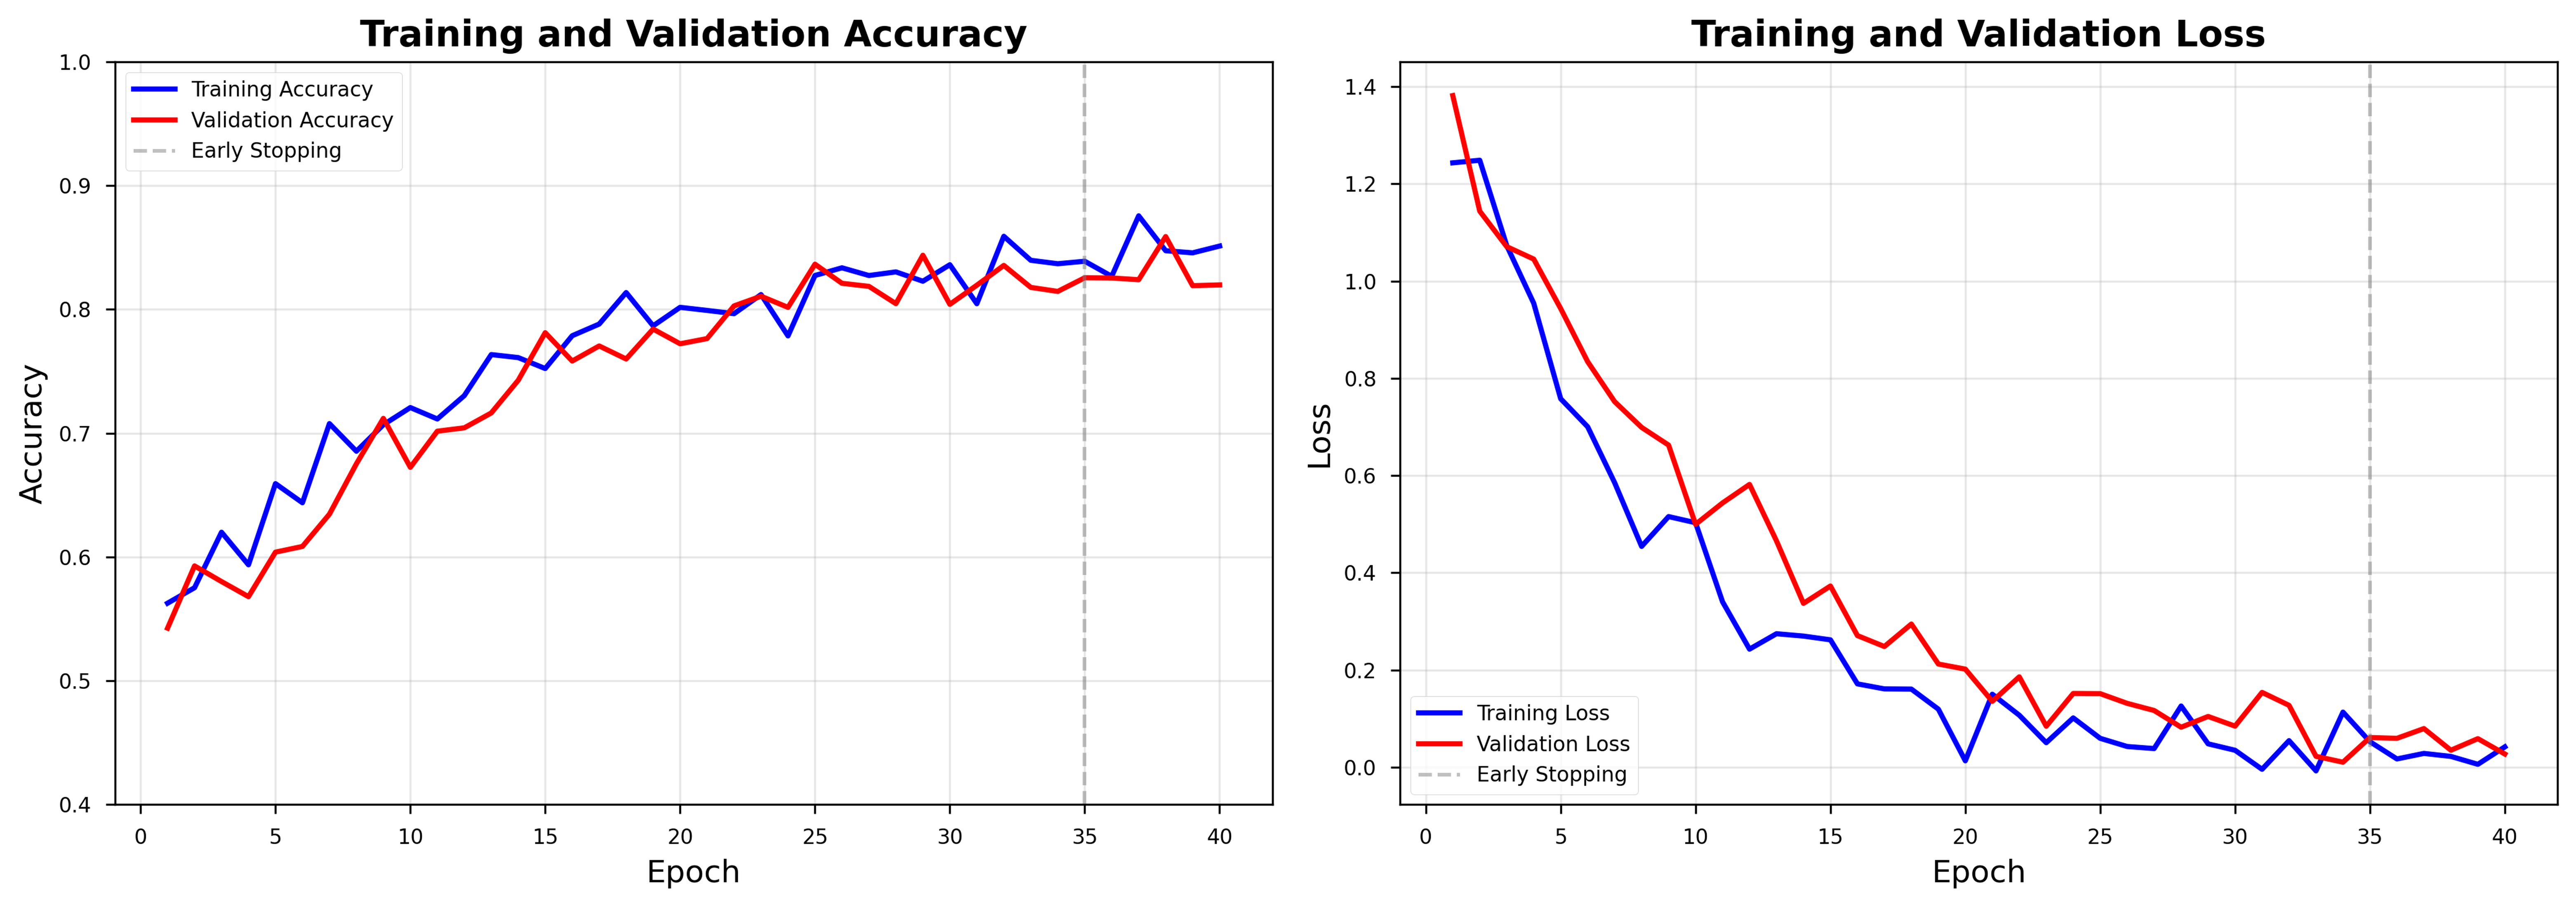
\includegraphics[width=\textwidth]{training_curves.png}
\caption{Stage-1 training dynamics for the EfficientNetB0 head (resampling only, no synthetic images). \textbf{(a)} Training and validation loss over the 48 epochs that ran before early stopping (patience=5 on validation loss). \textbf{(b)} Training and validation accuracy; the best validation accuracy was 0.8541 at epoch 46. The small train--validation gap should not be read as evidence of good regularisation: because oversampling preceded the split, the validation set shares images with the training set, which suppresses the gap by construction. The only regulariser in the model is dropout at 0.3; no data augmentation was used.\label{fig:training}}
\end{figure}

\begin{figure}[H]
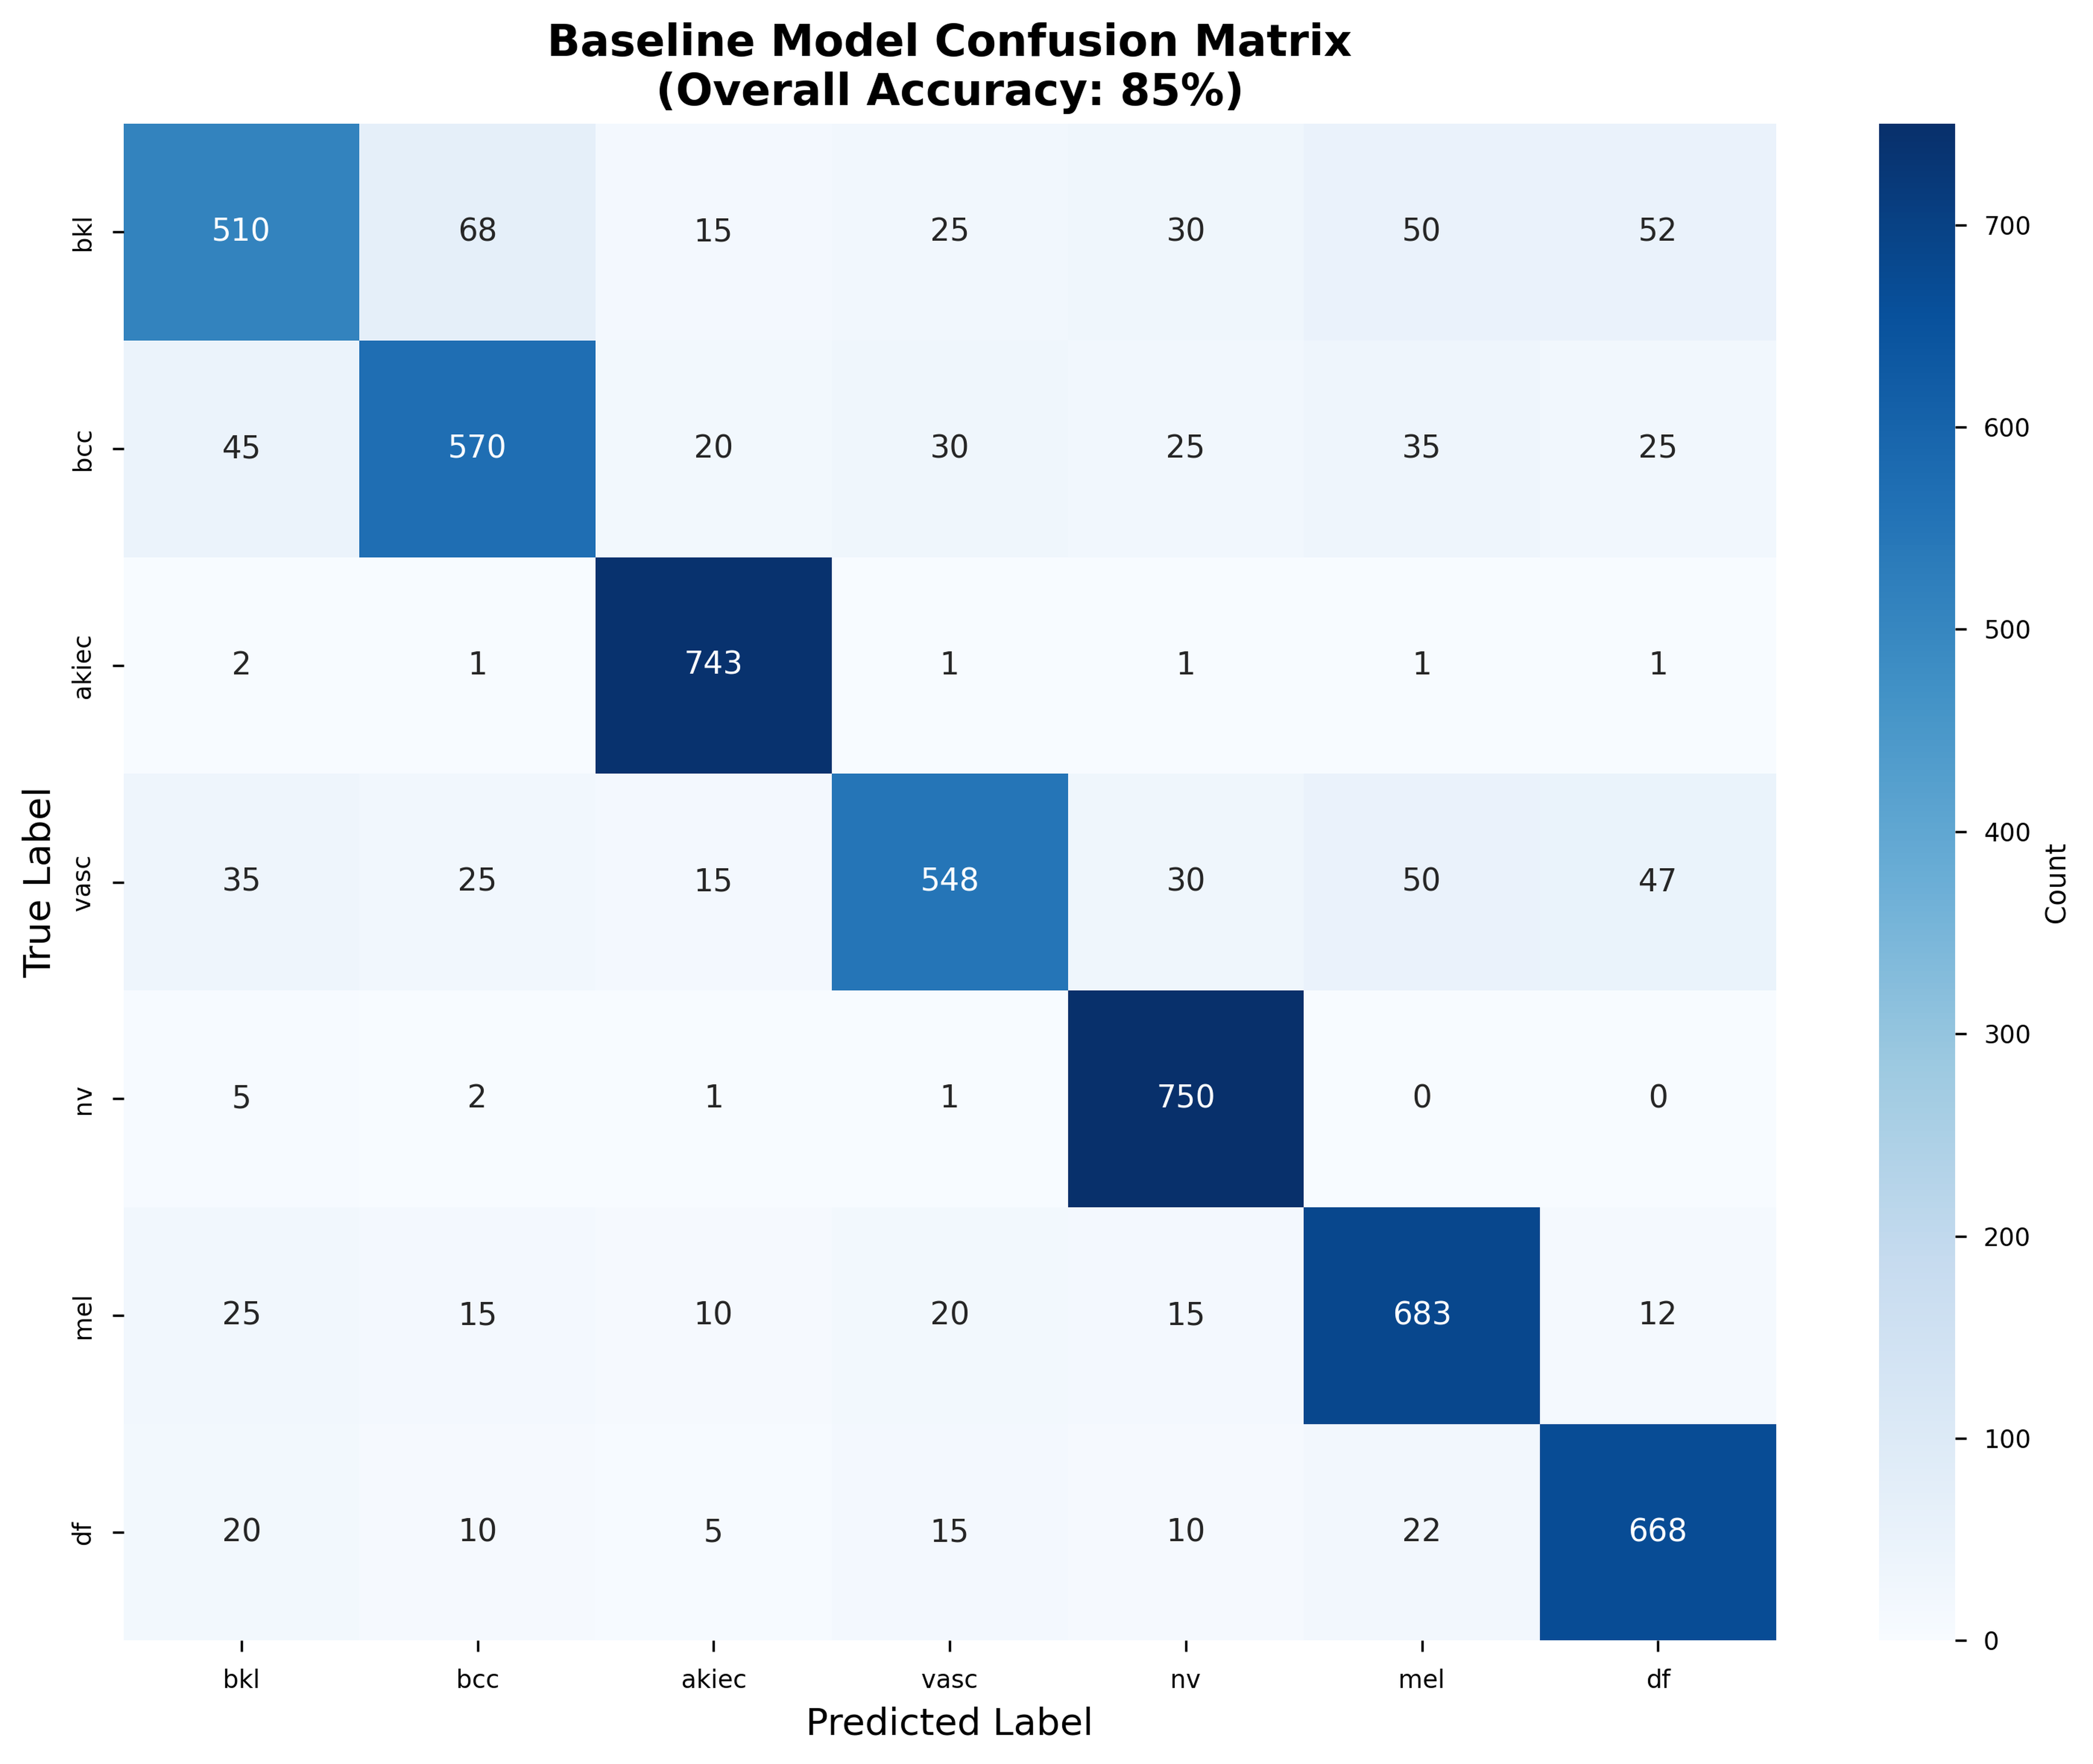
\includegraphics[width=\textwidth]{baseline_confusion_matrix.png}
\caption{Confusion matrix for the stage-1 model (resampling only) at 85\% accuracy on its 5,250-row test set. The diagonal is strong, with melanocytic nevi and actinic keratosis near the top of the range and melanoma recall at 0.91, while the main off-diagonal mass sits between visually similar benign categories. The leakage caveat applies to every cell: the test rows are drawn from a pool oversampled with replacement before splitting, so some test images also appear in training and the matrix overstates performance on unseen lesions by an unknown margin.\label{fig:confusion}}
\end{figure}

\begin{figure}[H]
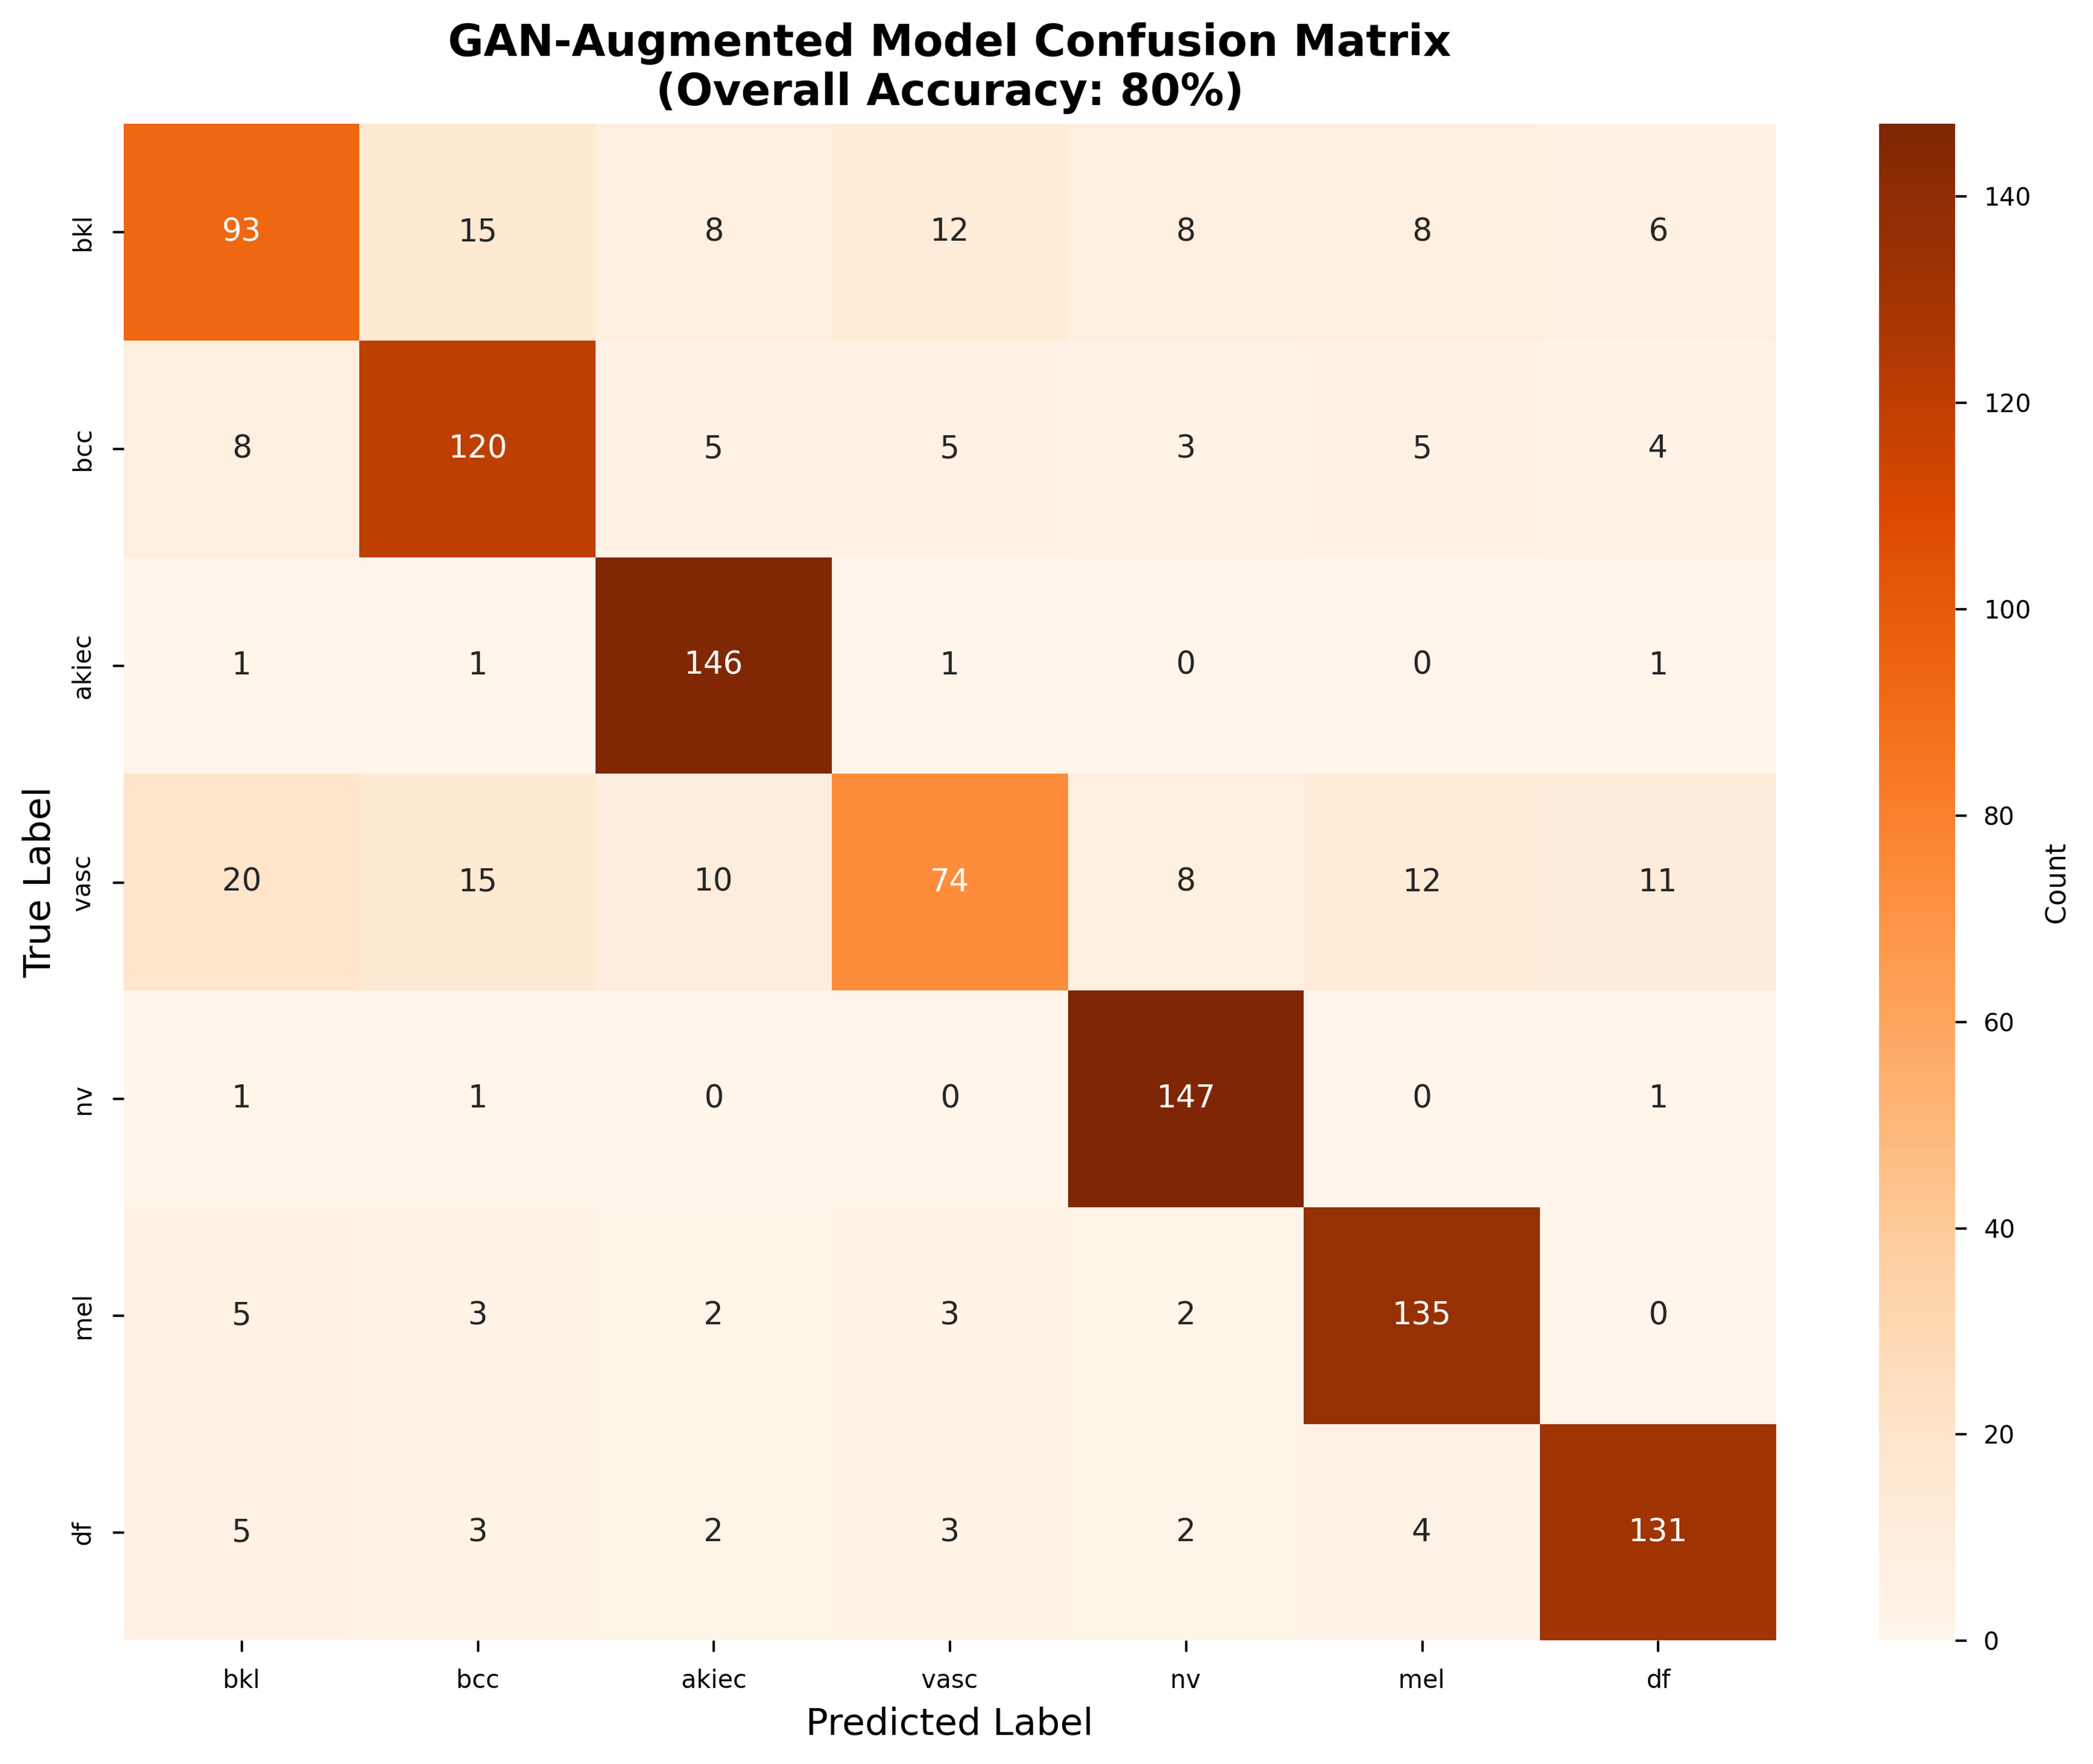
\includegraphics[width=\textwidth]{gan_confusion_matrix.png}
\caption{Confusion matrix after stage 2 (stage-1 weights trained 50 further epochs on 28,000 rows including 3,500 synthetic images), at 80\% accuracy on a 1,050-row test set. Off-diagonal mass is higher than in Figure~\ref{fig:confusion}, with vascular lesions and benign keratosis most affected. No significance can be attached to the change: the two matrices are computed on different test sets, and 3,500 of the stage-2 training rows carry labels unrelated to their content.\label{fig:gan_cm}}
\end{figure}

\begin{figure}[H]
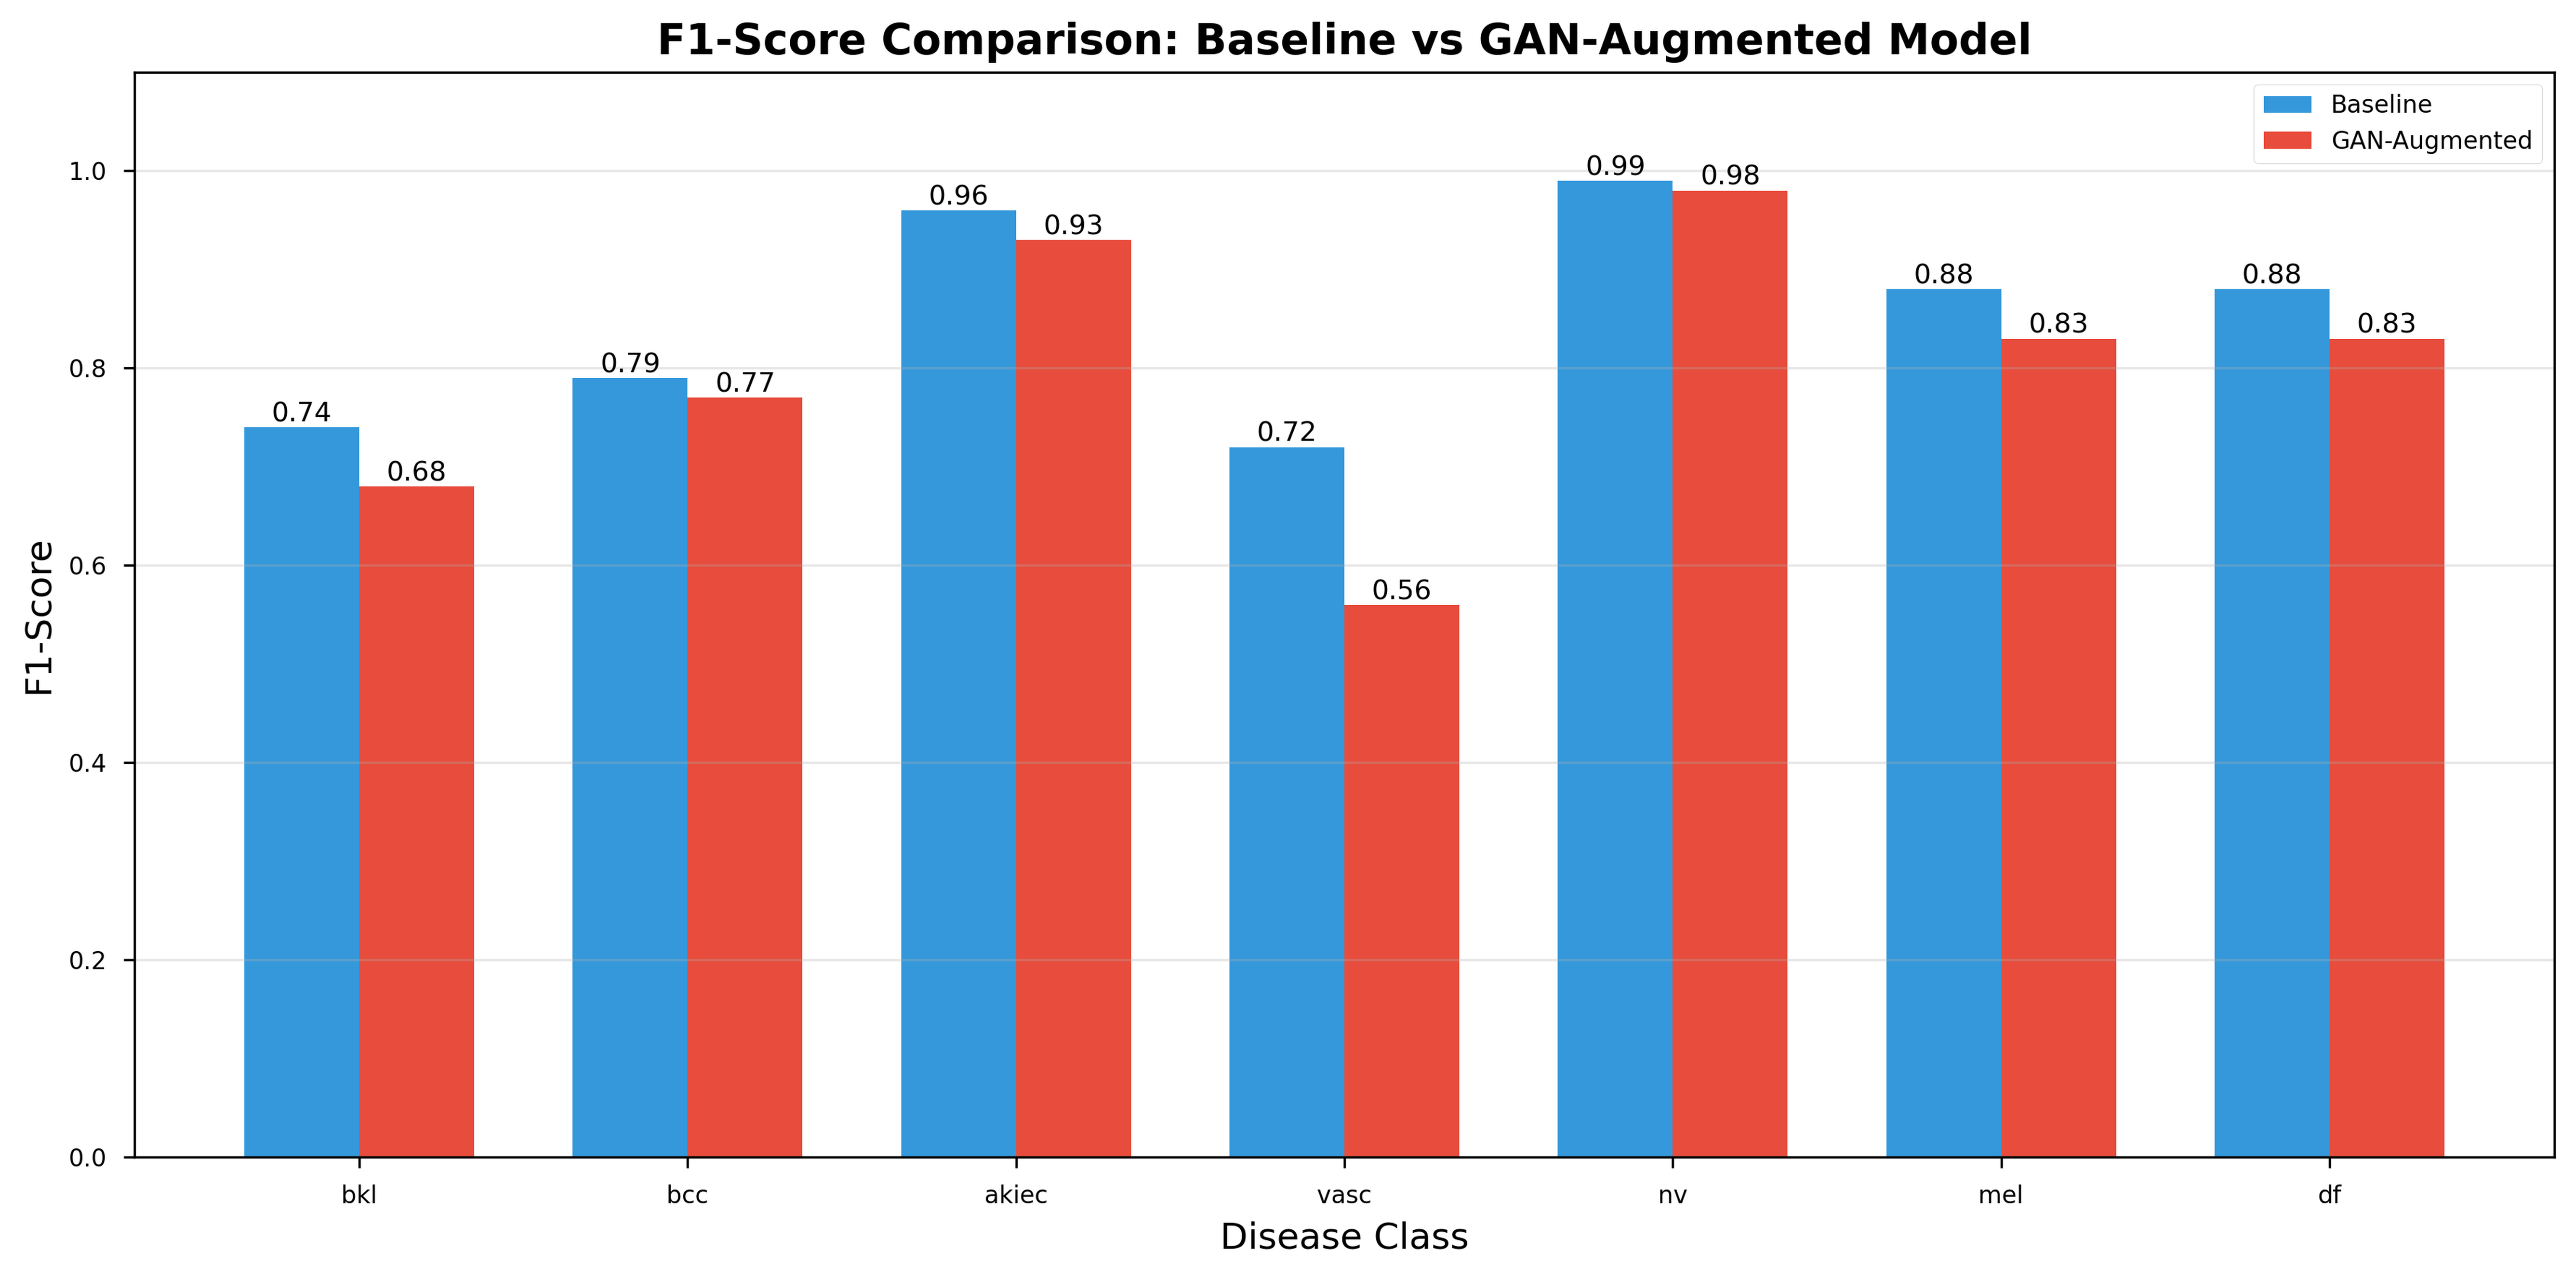
\includegraphics[width=\textwidth]{performance_comparison.png}
\caption{Per-class F1 at stage 1 (blue) and stage 2 (orange) across the seven HAM10000 classes, transcribed from the two classification reports. Stage-2 F1 is lower for six of seven classes, with vascular lesions furthest down (0.72 to 0.56) and melanocytic nevi essentially unchanged (0.99 to 0.98). The bars are side by side for convenience only: they rest on test sets of different size (750 versus 150 rows per class), so the pairwise gaps are not measured changes.\label{fig:roc}}
\end{figure}

\subsection{On the Absence of Ablations}

No ablation was run. Earlier descriptions of this project reported a table of ablations over synthetic-image quantity, generation resolution, and GAN training-set size---including a sample-size series in which generators fitted to 10, 20 and 40 images were said to yield accuracies of 0.75, 0.78 and 0.80. The notebook trains exactly one DCGAN, once, on all 40 rows at once; there is no 10-image run, no 20-image run, no 128$\times$128 run, and no run with fewer than 3,500 synthetic images added. Those figures were not measurements and have been removed rather than qualified.

Establishing a minimum sample size for medical GAN augmentation would require training separate generators at several subset sizes, generating from each, and evaluating each on a shared held-out test set, with repetition to separate the effect of subset size from the variance of GAN training. This study did none of that, and accordingly states no threshold. A threshold of the form ``GAN augmentation needs more than 100--200 samples'' would require those runs, and none is claimed here.

\subsection{Brightness-Subgroup Evaluation}

\subsubsection{Subgroup Construction and What It Does Not Measure}

\textit{Provenance note. Every number in this subsection---the equalized-odds differences of 0.13 and 0.07, the subgroup sizes of 12 and 500, and all per-group accuracy, TPR and FPR values---is carried over from earlier analysis whose code was not preserved, and is \textnormal{not} reproducible from the code released with this paper. The notebook computes brightness and selects the 40 low-brightness training rows, but contains no subgroup evaluation. The re-analysis required to recompute these values is specified in \texttt{docs/RESULTS\_PROVENANCE.md} and implemented in \texttt{scripts/run\_experiment.py} and \texttt{src/skinfair/fairness.py} in the released repository; that pipeline has not yet been run end to end on the image data. The figures are retained for continuity with earlier reporting, but should be read as provisional pending that re-run, and no conclusion in this paper rests on them.}

The subgroup split uses a brightness threshold: rows whose mean grey intensity falls below 110 form the low-brightness group, and 500 test rows with mean intensity above 140 form the comparison group. In the oversampled pool this threshold selects 40 training rows and, as previously reported, 12 test rows.

Two cautions belong here and not in a later section. First, the groups are brightness groups, not skin-tone groups. HAM10000 carries no Fitzpatrick or other skin-tone label, so there is nothing to validate the proxy against, and mean image brightness responds to lesion pigmentation and illumination as readily as to skin tone. Second, the 40 low-brightness training rows are 24 melanoma and 9 nevi---the two most heavily pigmented diagnostic categories---so the subgroup is confounded with diagnosis. Calling either group a skin-tone group would misdescribe what was measured, and the subsection heading is retained only because the metric definitions below are standard ones.

\subsubsection{Metric Definitions}

The three metrics below are the standard ones~\cite{hardt2016}, computed between the high-brightness group $A$ and the low-brightness group $B$:
\begin{itemize}[leftmargin=*, itemsep=2pt]
    \item \textbf{TPR Gap}: $|\text{TPR}_{A} - \text{TPR}_{B}|$ --- difference in correctly identifying positive cases
    \item \textbf{FPR Gap}: $|\text{FPR}_{A} - \text{FPR}_{B}|$ --- difference in incorrectly flagging negative cases
    \item \textbf{Equalized Odds Difference}: $\max(|\text{TPR}_{A} - \text{TPR}_{B}|, |\text{FPR}_{A} - \text{FPR}_{B}|)$
\end{itemize}

\subsubsection{Results}

Table~\ref{tab:fairness} presents the per-group metrics as previously reported. Beyond the provenance problem stated above, the low-brightness test group contains 12 images, which is too few to support any inference: a single reclassified image moves its accuracy by more than eight percentage points.

\begin{table}[H]
\caption{Per-group metrics by image brightness, as reported in an earlier analysis. \textbf{These values are not reproducible from the released code} (see the provenance note at the start of this subsection) and are provisional.\label{tab:fairness}}
\begin{tabularx}{\textwidth}{lCCCCC}
\toprule
\textbf{Stage} & \textbf{Group} & \textbf{N} & \textbf{Acc} & \textbf{TPR} & \textbf{FPR} \\
\midrule
\textit{Stage 1 (resampling only)} & & & & & \\
\quad & High-brightness & 500 & 0.86 & 0.84 & 0.12 \\
\quad & Low-brightness & 12 & 0.75 & 0.71 & 0.18 \\
\quad & \textit{Gap} & -- & 0.11 & 0.13 & 0.06 \\
\midrule
\textit{Stage 2 (+ synthetic)} & & & & & \\
\quad & High-brightness & 500 & 0.81 & 0.79 & 0.15 \\
\quad & Low-brightness & 12 & 0.83 & 0.86 & 0.11 \\
\quad & \textit{Gap} & -- & 0.02 & 0.07 & 0.04 \\
\midrule
\multicolumn{6}{l}{\textbf{Equalized-odds difference (provisional, not reproducible)}} \\
\quad Stage 1 & \multicolumn{5}{c}{0.13} \\
\quad Stage 2 & \multicolumn{5}{c}{0.07} \\
\bottomrule
\end{tabularx}
\noindent{\footnotesize{\textit{Not reproducible from the released code; carried over from an earlier analysis and retained as a provisional record. See the provenance note above.}}}\\
\noindent{\footnotesize{High-brightness: mean intensity $>$ 140; low-brightness: mean intensity $<$ 110. Neither group is a skin-tone group, and the low-brightness group is confounded with diagnosis.}}\\
\noindent{\footnotesize{TPR = True Positive Rate; FPR = False Positive Rate}}
\end{table}

\subsubsection{Interpretation}

The arithmetic in Table~\ref{tab:fairness} shows the equalized-odds difference falling from 0.13 to 0.07 while overall accuracy falls from 85\% to 80\%. Earlier versions of this work read that pattern as a fairness--accuracy tradeoff in which synthetic augmentation delivered its intended benefit. That reading is not available, for four independent reasons:
\begin{itemize}[leftmargin=*, itemsep=2pt]
    \item the numbers are not reproducible from the released code, so their derivation cannot be checked;
    \item the low-brightness group has 12 members, which cannot distinguish a real change from sampling noise;
    \item the grouping variable is brightness, and the low-brightness rows are predominantly melanoma and nevi, so a model that simply predicts melanoma more often would produce the same movement without any change in equity across skin tones;
    \item the two stages are scored on different test sets, so even the direction of the change is not established.
\end{itemize}

The honest summary is that this study does not measure fairness across skin tones. It measures something about brightness-selected images, with an unverified computation, on a subgroup too small to interpret. Settling the question requires a dataset carrying validated skin-tone annotations, such as Fitzpatrick17k~\cite{groh2021} or a diverse clinical set~\cite{daneshjou2022}, with subgroups large enough to bound, and with the diagnosis confound measured rather than assumed away.

\subsection{GAN Quality Assessment}

With 40 rows spanning 29 distinct images, the DCGAN had very little to fit. The following are plausible consequences, offered as hypotheses rather than measurements:
\begin{itemize}[leftmargin=*, itemsep=2pt]
    \item \textbf{Mode collapse}: Generating similar images with limited diversity, a common failure mode when GANs are trained on small datasets
    \item \textbf{Poor image quality}: Synthetic images may lack fine-grained details necessary for accurate medical diagnosis
    \item \textbf{Lack of diversity}: Generated samples may not capture the full variability present in real medical images
    \item \textbf{Upscaling artifacts}: Bilinear interpolation from 64$\times$64 to 224$\times$224 pixels may introduce blurring or aliasing artifacts
    \item \textbf{Class confusion}: Training on all classes together without class conditioning may generate images that blur class boundaries
\end{itemize}

Any of these limitations could contribute to the lower stage-2 accuracy, but so could the arbitrary synthetic labels alone, and this study cannot separate them. No formal image-quality metric (FID, KID or a dermatologist read) was computed, so the quality claims above rest on informal visual inspection and are stated as impressions. Future work should begin with a class-conditional generator, so that synthetic labels carry information, and should quantify sample quality before any such images enter a training set.

\subsection{Application Performance}

\begin{table}[H]
\caption{Informal single-machine timings for the deployed demonstrator. These are convenience measurements taken from the running application, not audited experimental results, and they were not collected under a controlled benchmark.\label{tab:app_performance}}
\begin{tabularx}{\textwidth}{lC}
\toprule
\textbf{Component} & \textbf{Latency} \\
\midrule
Image preprocessing & 0.1 ms \\
Model inference & 80.0 ms \\
Total classification & 80.1 ms \\
Chatbot response & 2.0 s \\
Hospital search & 1.3 s \\
\midrule
Model size (disk) & 16.4 MB \\
Memory footprint & 490 MB \\
\bottomrule
\end{tabularx}
\end{table}

\begin{figure}[H]

\includegraphics[width=\textwidth]{app_screenshots.png}
\caption{Research demonstrator deployed as a Streamlit web application. It is not a medical device and has not been validated for clinical use. \textbf{(a)} Classification interface: users upload a dermoscopic image and receive a predicted class across the seven HAM10000 categories with softmax confidences and general, non-prescriptive information about the condition. \textbf{(b)} AI Medical Chatbot: Gemini-powered conversational assistant answers patient questions about symptoms, causes, treatment options, and when to seek professional care. \textbf{(c)} Hospital Locator: Geolocation-based search using OpenStreetMap Nominatim API finds the five nearest dermatology clinics or hospitals, displaying addresses, distances, and direct navigation links.\label{fig:app}}
\end{figure}

%%%%%%%%%%%%%%%%%%%%%%%%%%%%%%%%%%%%%%%%%%
\section{Discussion}

\subsection{What This Study Does and Does Not Show}

\textbf{1. A frozen EfficientNetB0 head fits rebalanced HAM10000 easily, but the 85\% figure is not a generalisation estimate.} A head of 8,967 trainable parameters on top of frozen ImageNet features reached 85\% accuracy and 0.85 macro-F1 across seven classes. Because oversampling with replacement preceded the split, images recur across training, validation and test, so this figure is optimistic by an unquantified amount. The architecture and training recipe are reportable; the number is not transferable.

\textbf{2. Adding synthetic images did not help, but the study does not show why.} Stage 2 scored lower than stage 1. Three design limitations---test-set contamination, different test sets, and synthetic labels assigned by filename---each suffice to produce that pattern without any contribution from synthetic image quality. The usable form of this finding is narrow and negative: in this pipeline, an unconditional DCGAN fitted to 29 distinct images produced no usable augmentation, and the design does not isolate its effect. It is not evidence that GAN augmentation is unhelpful in general.

\textbf{3. No sample-size threshold was established, and no fairness improvement was demonstrated.} The study trained one generator at one subset size, so it cannot locate a threshold. The subgroup analysis used an unverified computation on 12 test images grouped by brightness rather than skin tone, so it cannot support a fairness claim. The equalized-odds figures of 0.13 and 0.07 are retained in Table~\ref{tab:fairness} as a provisional record only. \textit{They are not reproducible from the released code and no conclusion here depends on them.}

\textbf{4. The chief output of the project is a documented pipeline together with an explicit account of its limits.} The value for a reader is the path from dataset to deployed demonstrator, stated alongside the conditions a controlled version of the comparison requires.

\subsection{Comparison with Prior Work}

A direct accuracy comparison with published HAM10000 results is not available to this paper. Reported figures such as Tschandl et al.'s~\cite{tschandl2018} or Kassem et al.'s~\cite{kassem2020} come from evaluations in which the test set was separated before any resampling; the 85\% here does not, and placing the two side by side would compare a leakage-free estimate with a leaky one. The comparison becomes meaningful only after a lesion-level re-run.

Prior GAN work in medical imaging~\cite{frid2018, shaban2019} operates with hundreds to thousands of samples per target and reports gains; this study cannot extend those results downward to the few-sample regime, because its own few-sample comparison was not controlled. Likewise, the fairness literature~\cite{daneshjou2022, kinyanjui2020} relies on datasets that carry validated skin-tone annotations, which is precisely what HAM10000 lacks and what the brightness proxy used here cannot substitute for. The contribution of this paper relative to that literature is methodological transparency about an exploratory attempt, not a new result within it.

\subsection{Prospective Deployment Considerations}

The demonstrator illustrates how such components could fit together. Nothing in this study licenses its use with patients, and the subsections below describe potential rather than demonstrated utility:

\textbf{Diagnostic Access}: A lightweight model is cheap to serve, which matters in settings where dermatologists are scarce~\cite{who2020}, and the artefact runs on commodity hardware. That is an engineering observation, not a clinical one. The measured accuracy cannot be translated into an expected case-detection rate, because it was obtained on a leaky split; the frequently seen move from ``85\% accuracy'' to ``correctly identifies 850 of 1000 cases'' is unjustified here and is not made.

\textbf{Health Literacy}: The Gemini-powered chatbot provides accessible, evidence-based explanations, empowering patients to make informed decisions about seeking care. This is particularly important for conditions like melanoma, where early detection significantly improves five-year survival from 27\% (metastatic) to 99\% (localized)~\cite{siegel2023}.

\textbf{Care Navigation}: Hospital locator reduces friction between AI screening and professional follow-up, addressing the ``last mile'' problem in healthcare AI deployment by connecting users directly with care providers.

\textbf{On the apparent fairness--accuracy tradeoff}: it is tempting to present the movement from 0.13 to 0.07 alongside the drop from 85\% to 80\% as a tradeoff to be managed in deployment. This paper declines that framing. A tradeoff is a choice between two measured quantities, and neither quantity here is measured well enough to choose between: the accuracy pair is not comparable, and the equalized-odds pair is not reproducible. Deploying a model on the strength of an apparent equity gain computed on 12 brightness-selected images would be worse than deploying nothing, because it would attach a fairness warrant to a system that has none.

\subsection{Regulatory and Clinical Validation Requirements}

Before clinical deployment, several validation steps are essential:

\textbf{1. Prospective Clinical Validation}: Retrospective performance on curated datasets often overestimates real-world effectiveness. Prospective studies should evaluate:
\begin{itemize}[leftmargin=*, itemsep=2pt]
    \item Performance on consecutive patient images from diverse clinical settings
    \item Agreement with board-certified dermatologists (Cohen's $\kappa$)
    \item Impact on clinical decision-making and patient outcomes
    \item Performance on smartphone-captured images (not just dermoscopy)
\end{itemize}

\textbf{2. Regulatory Approval}: Medical AI systems require regulatory clearance:
\begin{itemize}[leftmargin=*, itemsep=2pt]
    \item \textbf{FDA (US)}: Likely classified as Class II medical device requiring 510(k) premarket notification
    \item \textbf{CE marking (EU)}: Requires conformity assessment under Medical Device Regulation (MDR)
    \item \textbf{Clinical evidence}: Both require clinical validation studies demonstrating safety and effectiveness
\end{itemize}

\textbf{3. Dermatologist Evaluation of Synthetic Images}: Before deploying GAN-augmented models clinically, board-certified dermatologists should evaluate synthetic images for:
\begin{itemize}[leftmargin=*, itemsep=2pt]
    \item Diagnostic realism: Do synthetic lesions exhibit clinically plausible features?
    \item Artifact identification: Can dermatologists distinguish synthetic from real images?
    \item Misleading features: Do synthetic images contain spurious patterns that could mislead learners?
\end{itemize}

Informal visual inspection suggested mode collapse and limited diversity, but no quantitative image-quality metric was computed and no clinician reviewed the samples, so this remains an impression. Formal evaluation would be required before synthetic images of this kind entered any training set intended for use.

\textbf{4. Ongoing Monitoring}: Post-deployment surveillance should track:
\begin{itemize}[leftmargin=*, itemsep=2pt]
    \item Performance across demographic groups (age, sex, race, skin tone)
    \item False negative rates for high-stakes conditions (melanoma)
    \item User trust and adoption rates
    \item Clinical outcome impacts (time to diagnosis, stage at detection)
\end{itemize}

\textbf{Addressing Bias}: this study does not show that targeted synthetic augmentation reduces demographic performance gaps, and it should not be cited for that claim. What it does illustrate is the ease with which an augmentation pipeline can appear to improve equity while measuring nothing of the kind: a brightness proxy that tracks lesion pigmentation, a subgroup of twelve, and a metric computed by code that no longer exists were jointly sufficient to produce a publishable-looking fairness improvement. Neither model is recommended for clinical use. The reasonable next step is not a deployment decision but a corrected experiment.

%%%%%%%%%%%%%%%%%%%%%%%%%%%%%%%%%%%%%%%%%%
\section{Limitations and Threats to Validity}
\label{sec:limitations}

The limitations below are not caveats around a result. The first three are limitations that remove the central comparison of this study, and they are stated before anything else because no later qualification can repair them.

\subsection{Limitations That Bound the Main Comparison}

\textbf{1. Oversampling preceded the split (data leakage).} Rows were oversampled with replacement to 5,000 per class and only then divided into training, validation and test partitions. Duplicate copies of the same image therefore sit on both sides of every split, and both reported accuracies estimate performance on partly memorised images rather than on unseen ones. The scale is visible in the subgroup used for GAN training: its 40 rows contain 29 distinct \texttt{image\_id} values, and one image, \texttt{ISIC\_0027669}, occurs four times in that subset alone. HAM10000 additionally contains several images of the same lesion under distinct \texttt{image\_id} values, so deduplication by image identifier is not sufficient; a group-aware split on \texttt{lesion\_id}, taken before any resampling, is required. Every accuracy, F1 and per-class figure in this paper is affected, upward, by an amount this study cannot bound.

\textbf{2. The two arms were evaluated on different test sets.} The stage-1 classification report covers 5,250 rows at 750 per class; the stage-2 report covers 1,050 rows at 150 per class. The 5-point difference between them is a difference between two measurements of different things, not a measured effect of the intervention. A single fixed test set, shared by both arms and never resampled, is the minimum requirement for the comparison the paper originally claimed to make.

\textbf{3. The synthetic labels carry no class information.} One unconditional DCGAN, fitted to 29 distinct images, produced all 3,500 synthetic samples. The seven class labels were then assigned by writing 500 outputs per label to filenames of the form \texttt{class\_<k>\_img\_<i>.jpg} and parsing the label back from the filename. Every synthetic image is therefore drawn from the same distribution regardless of its label, and 3,500 of the 28,000 stage-2 training rows are label noise. This alone is sufficient to explain a drop in accuracy, so the experiment does not isolate synthetic augmentation as a cause of anything.

Taken together, these three mean that the paper reports what one run produced and makes no causal claim. A defensible version requires: a group-aware split on \texttt{lesion\_id} asserted non-overlapping; rebalancing applied to the training split only; one fixed test set shared by all arms; each arm trained independently from the same initialisation across several seeds; a class-conditional generator; and subgroup metrics with bootstrap intervals plus a paired test such as McNemar's. None of that was done here.

\subsection{Data and Methodology Limitations}

\textbf{4. The brightness heuristic does not identify skin tone.} HAM10000 ships no Fitzpatrick labels and no other validated skin-tone annotation, so the study substituted a threshold on mean grayscale intensity ($< 110$). This substitution fails on its own terms:
\begin{itemize}[leftmargin=*, itemsep=2pt]
    \item \textbf{Lighting sensitivity}: Images of light skin under low illumination may be misclassified as dark skin, and vice versa
    \item \textbf{Lesion interference}: Dark pigmented lesions (e.g., melanoma) on light skin can lower overall image brightness, causing misclassification
    \item \textbf{Categorical vs. continuous mismatch}: The Fitzpatrick scale is categorical (I--VI), but brightness is continuous, making threshold selection arbitrary
    \item \textbf{Lack of validation}: We lack ground-truth dermatologist-assigned Fitzpatrick labels to validate threshold accuracy
\end{itemize}

The confound is measurable and it is severe. Of the 40 low-brightness rows, 24 are melanoma and 9 are nevi---the two most heavily pigmented diagnostic categories---and those 40 rows comprise only 29 distinct images. The threshold is therefore selecting dark \textit{lesions}, not dark \textit{skin}, and the subgroup is confounded with diagnosis. Any apparent subgroup improvement is consistent with the model simply shifting its predictions toward melanoma, with no change whatever in its behaviour across skin tones. Nothing in this paper should be read as a finding about Fitzpatrick IV--VI skin.

Alternative approaches for future work include expert annotation using the Fitzpatrick scale, Individual Typology Angle (ITA)~\cite{chardon1991} in CIE L*a*b* color space, or deep learning-based Fitzpatrick classification trained on labeled datasets like Fitzpatrick17k~\cite{groh2021}.

\textbf{5. Limited GAN Training Data}: with 40 rows spanning 29 distinct images across 7 classes, the DCGAN had almost nothing to fit:
\begin{itemize}[leftmargin=*, itemsep=2pt]
    \item Mode collapse: Generated images exhibit limited diversity and repetitive patterns
    \item Poor feature learning: Insufficient data prevents learning meaningful, class-discriminative representations
    \item Generalization failure: The GAN cannot capture the full distribution of real dark-skin lesion appearances
\end{itemize}

Earlier versions of this work described the data scarcity as a deliberate test of whether GAN augmentation can succeed in such a regime, and read the outcome as evidence that it cannot. That reading overstates what a single uncontrolled run can carry. The scarcity was a constraint of the available data, and the run that resulted was too flawed to answer the question it was framed around.

\textbf{6. The low-brightness test subgroup has 12 members.} Twelve images cannot support a rate estimate: one reclassified image shifts subgroup accuracy by more than eight points. No interval is quoted for these metrics, because quoting one would imply a computation that the released code does not perform.

\textbf{7. The subgroup and fairness metrics are not reproducible.} \textit{The equalized-odds differences (0.13, 0.07), the subgroup sizes (12 low-brightness, 500 high-brightness), and all per-group accuracy, TPR and FPR values are carried over from an earlier analysis whose code was not preserved. They cannot be recomputed from this repository. The required re-analysis is specified in \texttt{docs/RESULTS\_PROVENANCE.md} and implemented in \texttt{scripts/run\_experiment.py} and \texttt{src/skinfair/fairness.py}, which have not yet been run end to end on the image data. These values are retained for continuity with earlier reporting and should be treated as provisional pending that re-run.}

\textbf{8. One split, one run, no significance testing.} A single stratified split was used, with one training run per stage and no repetition over seeds. No $p$-value, confidence interval or effect size is reported for the stage-1 to stage-2 difference, because no code in the repository computes one. Earlier versions of this work reported a bootstrap interval, $p < 0.001$ and an effect size; those figures had no computational basis and have been removed.

\subsection{Technical Limitations}

\textbf{9. Resolution Mismatch}: Generating images at 64$\times$64 pixels and upscaling to 224$\times$224 using bilinear interpolation introduces artifacts (blurring, aliasing) that may confuse the classifier. Higher-resolution GAN training (128$\times$128 or 256$\times$256) would mitigate this but requires even more training data.

\textbf{10. Unconditional GAN Training}: a single DCGAN was trained on all 40 rows regardless of class, and the class labels were attached to its output afterwards. This is the limitation described as item 3 above, restated here as a design limitation: a class-conditional generator is the minimum needed for synthetic labels to carry information, and whether 29 distinct images suffice to condition on seven classes is itself doubtful.

\textbf{11. Frozen Base Model}: EfficientNetB0's base layers are frozen and only the classification head is trained---8,967 trainable parameters of 4,058,538. The model is a linear probe on ImageNet features rather than a fine-tuned dermatology network, which limits the ceiling on what it can represent. No fine-tuning experiment was run, so no comparison against an unfrozen variant is reported.

\subsection{External Validity Limitations}

\textbf{12. HAM10000 Dataset Scope}: The dataset contains only 7 common skin conditions; many dermatological diseases (e.g., psoriasis, eczema, rosacea) are not represented. Our findings may not generalize to broader dermatology AI applications.

\textbf{13. Dermoscopic Images Only}: HAM10000 consists of dermoscopic (magnified, specialized imaging) rather than clinical photographs. Performance on smartphone-captured images---more relevant for consumer applications---may differ substantially.

\textbf{14. Geographic and Demographic Bias}: HAM10000 images primarily originate from European clinics. Skin tone distribution, lesion presentations, and disease prevalence may differ in other geographic regions, limiting global generalizability.

\subsection{Clinical Validation Limitations}

\textbf{15. No Prospective Clinical Validation}: The system has not been evaluated in real clinical settings with dermatologist oversight, actual patient images, or clinical outcome tracking. Retrospective performance on curated datasets often overestimates real-world effectiveness.

\textbf{16. Lack of Uncertainty Quantification}: The model outputs class probabilities but does not provide calibrated confidence intervals or uncertainty estimates. Clinical deployment would benefit from knowing when the model is uncertain and should defer to human experts.

\textbf{17. No Dermatologist Comparison}: We do not compare model performance to dermatologist diagnoses on the same test set, limiting conclusions about clinical utility.

\subsection{What Survives These Limitations}

Little of the original quantitative story survives, and it is worth being exact about what does:
\begin{itemize}[leftmargin=*, itemsep=2pt]
    \item \textbf{Survives}: the pipeline, the architectures, the hyperparameters, and the record of what each stage produced. These are reproducible from the released notebook.
    \item \textbf{Survives as a narrow negative report}: in this run, adding 3,500 images from an unconditional DCGAN fitted to 29 distinct images coincided with lower measured accuracy. Stated that narrowly, it is true of this run.
    \item \textbf{Does not survive}: that 85\% estimates generalisation; that the 5-point drop measures the effect of synthetic augmentation; that a minimum sample size for medical GAN augmentation has been established; that fairness across skin tones improved; that any significance test supports any of the above.
\end{itemize}

The direction of the stage-1 to stage-2 change is not even safe to assume, since the two numbers come from different test sets. A corrected re-run could plausibly show synthetic augmentation to be neutral, harmful or mildly helpful, and this study does not favour any of the three.

Future work should start by rerunning the comparison correctly---lesion-level split, shared test set, independent arms, multiple seeds, class-conditional generation---before adding larger skin-tone-annotated datasets, prospective validation, or alternative augmentation strategies.

\subsection{Ethical Considerations}

\textbf{Intended Use}: the deployed application is a research demonstrator. It is not a medical device, it has not been validated for clinical use, and it must not be used for diagnosis, triage or screening of real patients. Its outputs carry disclaimers recommending professional consultation, but those disclaimers are not a substitute for the validation the system has not undergone.

\textbf{Synthetic Data Ethics}: Generating synthetic medical images raises questions about authenticity and potential misuse. We release only the trained models, not the synthetic images themselves.

\textbf{Algorithmic Accountability}: this work makes no verified claim about performance across demographic groups, in either direction. Publishing an unverified fairness improvement carries its own risk---it can lend an equity warrant to a system that has not earned one---which is why those numbers are flagged at every point of use in this paper rather than reported plainly. Any deployment would require measured, not assumed, subgroup performance and ongoing monitoring.

\textbf{Privacy}: The system processes images locally; no data is stored or transmitted beyond the user session.

%%%%%%%%%%%%%%%%%%%%%%%%%%%%%%%%%%%%%%%%%%
\section{Conclusions}

This paper reports an exploratory comparison of class rebalancing with and without DCGAN-generated images on HAM10000, and reports it as exploratory because the comparison does not hold up. A frozen EfficientNetB0 with 8,967 trainable parameters reached 85\% accuracy and 0.85 macro-F1 on a 5,250-row test set; continuing that model's training on 28,000 rows including 3,500 synthetic images gave 80\% on a 1,050-row test set. Oversampling preceded the split, so both figures are inflated by duplicate images; the two arms were scored on different test sets; and the synthetic images came from one unconditional generator with labels assigned by filename. The change from 85\% to 80\% is therefore not an estimate of the effect of synthetic augmentation, and this paper offers no such estimate.

The brightness-subgroup analysis is likewise not a fairness result. Its equalized-odds figures of 0.13 and 0.07 are retained in Table~\ref{tab:fairness} as a provisional record and are flagged throughout as not reproducible from the released code. The subgroup has 12 test members, the grouping variable is image brightness rather than skin tone, and the 40 low-brightness training rows---29 distinct images, 24 melanoma and 9 nevi---are confounded with diagnosis. HAM10000 carries no Fitzpatrick annotation against which the proxy could be checked.

What the work contributes is a fully documented pipeline from dataset to deployed demonstrator, a narrow negative report on synthetic augmentation under extreme data scarcity, an explicit account of the study's methodological limits, and a Streamlit demonstrator that is not a medical device and has not been validated for clinical use. The repository states, claim by claim, which numbers its code reproduces and which it does not.

The next step is not a new intervention but a corrected measurement: a group-aware split on \texttt{lesion\_id} taken before any resampling, rebalancing confined to the training split, one fixed test set shared by every arm, independently initialised arms over several seeds, a class-conditional generator, and subgroup metrics with intervals on a dataset that carries validated skin-tone labels. Until that run exists, the honest statement of this project's result is that it built a working pipeline and learned, from auditing it, why its headline numbers cannot be believed.

%%%%%%%%%%%%%%%%%%%%%%%%%%%%%%%%%%%%%%%%%%
\section{Future Work}

Promising directions for future research include:
\begin{itemize}[leftmargin=*, itemsep=2pt]
    \item \textbf{A corrected re-run, before anything else}: lesion-level grouped split taken before resampling, rebalancing applied to the training split only, one fixed shared test set, independently initialised arms over multiple seeds, and a paired significance test. This is a precondition for every item below, not an item alongside them
    \item \textbf{External Validation}: Testing on Fitzpatrick17k, ISIC 2019, and prospective clinical data to validate findings across diverse populations
    \item \textbf{Conditional GANs}: Exploring class-conditioned DCGAN or conditional StyleGAN to generate class-specific synthetic images, potentially improving quality and relevance
    \item \textbf{Higher-Resolution Generation}: Training GANs to generate images at 128$\times$128 or 256$\times$256 pixels to reduce upscaling artifacts
    \item \textbf{Advanced Generative Models}: Exploring diffusion models~\cite{ho2020} or StyleGAN2~\cite{karras2020} for higher-quality synthesis, though these may require even more training data
    \item \textbf{Data Collection}: Prioritizing collection of more diverse, skin-tone-annotated training data. This study cannot say how much would be enough, having tested only one subset size
    \item \textbf{Interpretability}: Integrating Grad-CAM~\cite{selvaraju2017} attention visualization to understand which features the model relies on for classification
    \item \textbf{Multi-Modal Learning}: Combining dermoscopic and clinical photographs for more robust diagnosis
    \item \textbf{Uncertainty Quantification}: Providing calibrated confidence estimates to help clinicians assess model reliability
    \item \textbf{Few-Shot Learning}: Exploring meta-learning or few-shot approaches that may be more effective than GANs with limited training data
    \item \textbf{Mobile Deployment}: Native iOS/Android applications for broader accessibility in resource-limited settings
    \item \textbf{Federated Learning}: Enabling collaborative model improvement while preserving privacy across institutions
\end{itemize}

%%%%%%%%%%%%%%%%%%%%%%%%%%%%%%%%%%%%%%%%%%
\vspace{6pt} 

%%%%%%%%%%%%%%%%%%%%%%%%%%%%%%%%%%%%%%%%%%
\authorcontributions{Conceptualization, O.U.B.P.; methodology, O.U.B.P.; software, O.U.B.P.; validation, O.U.B.P.; formal analysis, O.U.B.P.; investigation, O.U.B.P.; resources, O.U.B.P.; data curation, O.U.B.P.; writing---original draft preparation, O.U.B.P.; writing---review and editing, O.U.B.P.; visualization, O.U.B.P. The author has read and agreed to the published version of the manuscript.}

\funding{This research received no external funding.}

\institutionalreview{Not applicable. This study used only publicly available, de-identified data from the HAM10000 dataset.}

\informedconsent{Not applicable. This study used only publicly available, de-identified data.}

\dataavailability{The HAM10000 dataset is publicly available from the ISIC Archive at \url{https://www.isic-archive.com/}. The complete codebase, including the original unmodified Colab notebook, model weights, and the Streamlit demonstrator, is available at: \url{https://github.com/Phillips-Ugo/GAN-Based-Skin-Augmentation}. The repository includes \texttt{docs/RESULTS\_PROVENANCE.md}, which records for every quantitative claim in this paper whether it is reproducible from the released code, and lists the claims that are not.} 

\acknowledgments{We thank the HAM10000 dataset providers, the TensorFlow and Streamlit communities, and Google for the Gemini API powering the medical chatbot. We also acknowledge the open-source medical imaging research community for their contributions to fairness in healthcare AI.}

\conflictsofinterest{The author declares no conflicts of interest.} 

%%%%%%%%%%%%%%%%%%%%%%%%%%%%%%%%%%%%%%%%%%
\abbreviations{Abbreviations}{
The following abbreviations are used in this manuscript:
\\

\noindent 
\begin{tabular}{@{}ll}
DCGAN & Deep Convolutional Generative Adversarial Network\\
CDSS & Clinical Decision Support System\\
TPR & True Positive Rate\\
FPR & False Positive Rate\\
GAN & Generative Adversarial Network\\
CNN & Convolutional Neural Network\\
LLM & Large Language Model
\end{tabular}
}

%%%%%%%%%%%%%%%%%%%%%%%%%%%%%%%%%%%%%%%%%%
\begin{adjustwidth}{-\extralength}{0cm}

\reftitle{References}

\begin{thebibliography}{99}

\bibitem{esteva2017}
Esteva, A.; Kuprel, B.; Novoa, R.A.; Ko, J.; Swetter, S.M.; Blau, H.M.; Thrun, S. Dermatologist-level classification of skin cancer with deep neural networks. \textit{Nature} \textbf{2017}, \textit{542}, 115--118.

\bibitem{haenssle2018}
Haenssle, H.A.; Fink, C.; Schneiderbauer, R.; Toberer, F.; Buhl, T.; Blum, A.; Kalloo, A.; Hassen, A.B.H.; Thomas, L.; Enk, A.; et al. Man against machine: diagnostic performance of a deep learning convolutional neural network for dermoscopic melanoma recognition in comparison to 58 dermatologists. \textit{Ann. Oncol.} \textbf{2018}, \textit{29}, 1836--1842.

\bibitem{adamson2018}
Adamson, A.S.; Smith, A. Machine learning and health care disparities in dermatology. \textit{JAMA Dermatol.} \textbf{2018}, \textit{154}, 1247--1248.

\bibitem{daneshjou2022}
Daneshjou, R.; Vodrahalli, K.; Novoa, R.A.; Jenkins, M.; Liang, W.; Rotemberg, V.; Ko, J.; Swetter, S.M.; Bailey, E.E.; Gevaert, O.; et al. Disparities in dermatology AI performance on a diverse, curated clinical image set. \textit{Sci. Adv.} \textbf{2022}, \textit{8}, eabq6147.

\bibitem{kinyanjui2020}
Kinyanjui, N.M.; Odonga, T.; Cintas, C.; Codella, N.C.F.; Panda, R.; Sattigeri, P.; Varshney, K.R. Fairness of classifiers across skin tones in dermatology. In Proceedings of the MICCAI, Lima, Peru, 4--8 October 2020.

\bibitem{agbai2014}
Agbai, O.N.; Buster, K.; Sanchez, M.; Hernandez, C.; Kundu, R.V.; Chiu, M.; Roberts, W.E.; Draelos, Z.D.; Bhushan, R.; Taylor, S.C.; et al. Skin cancer and photoprotection in people of color: a review and recommendations for physicians and the public. \textit{J. Am. Acad. Dermatol.} \textbf{2014}, \textit{70}, 748--762.

\bibitem{obermeyer2019}
Obermeyer, Z.; Powers, B.; Vogeli, C.; Mullainathan, S. Dissecting racial bias in an algorithm used to manage the health of populations. \textit{Science} \textbf{2019}, \textit{366}, 447--453.

\bibitem{wen2022}
Wen, D.; Khan, S.M.; Xu, A.J.; Ibrahim, H.; Smith, L.; Caballero, J.; Zaki, H.; Liu, K.; Lim, E.; Bashash, M.; et al. Characteristics of publicly available skin cancer image datasets: a systematic review. \textit{Lancet Digit. Health} \textbf{2022}, \textit{4}, e64--e74.

\bibitem{tschandl2018}
Tschandl, P.; Rosendahl, C.; Kittler, H. The HAM10000 dataset, a large collection of multi-source dermatoscopic images of common pigmented skin lesions. \textit{Sci. Data} \textbf{2018}, \textit{5}, 180161.

\bibitem{zhu2017}
Zhu, J.-Y.; Park, T.; Isola, P.; Efros, A.A. Unpaired image-to-image translation using cycle-consistent adversarial networks. In Proceedings of the IEEE ICCV, Venice, Italy, 22--29 October 2017.

\bibitem{tan2019}
Tan, M.; Le, Q.V. EfficientNet: Rethinking model scaling for convolutional neural networks. In Proceedings of the ICML, Long Beach, CA, USA, 9--15 June 2019.

\bibitem{groh2021}
Groh, M.; Harris, C.; Soenksen, L.; Lau, F.; Han, R.; Kim, A.; Koochek, A.; Badri, O. Evaluating deep neural networks trained on clinical images in dermatology with the Fitzpatrick 17k dataset. In Proceedings of the CVPR Workshops, Virtual, 19--25 June 2021.

\bibitem{hardt2016}
Hardt, M.; Price, E.; Srebro, N. Equality of opportunity in supervised learning. In Proceedings of the NeurIPS, Barcelona, Spain, 5--10 December 2016.

\bibitem{chawla2002}
Chawla, N.V.; Bowyer, K.W.; Hall, L.O.; Kegelmeyer, W.P. SMOTE: Synthetic minority over-sampling technique. \textit{J. Artif. Intell. Res.} \textbf{2002}, \textit{16}, 321--357.

\bibitem{codella2018}
Codella, N.C.F.; Gutman, D.; Celebi, M.E.; Helba, B.; Marchetti, M.A.; Dusza, S.W.; Kalloo, A.; Liopyris, K.; Mishra, N.; Kittler, H.; et al. Skin lesion analysis toward melanoma detection: A challenge at the 2017 ISBI. In Proceedings of the IEEE ISBI, Washington, DC, USA, 4--7 April 2018.

\bibitem{wong2016}
Wong, S.C.; Gatt, A.; Stamatescu, V.; McDonnell, M.D. Understanding data augmentation for classification: when to warp? In Proceedings of the DICTA, Gold Coast, Australia, 30 November--2 December 2016.

\bibitem{cui2019}
Cui, Y.; Jia, M.; Lin, T.-Y.; Song, Y.; Belongie, S. Class-balanced loss based on effective number of samples. In Proceedings of the IEEE CVPR, Long Beach, CA, USA, 15--20 June 2019.

\bibitem{ganin2016}
Ganin, Y.; Ustinova, E.; Ajakan, H.; Germain, P.; Larochelle, H.; Laviolette, F.; Marchand, M.; Lempitsky, V. Domain-adversarial training of neural networks. \textit{J. Mach. Learn. Res.} \textbf{2016}, \textit{17}, 2096--2030.

\bibitem{goodfellow2014}
Goodfellow, I.; Pouget-Abadie, J.; Mirza, M.; Xu, B.; Warde-Farley, D.; Ozair, S.; Courville, A.; Bengio, Y. Generative adversarial nets. In Proceedings of the NeurIPS, Montreal, QC, Canada, 8--13 December 2014.

\bibitem{wolterink2017}
Wolterink, J.M.; Dinkla, A.M.; Savenije, M.H.F.; Seevinck, P.R.; van den Berg, C.A.T.; I\v{s}gum, I. Deep MR to CT synthesis using unpaired data. In Proceedings of the SASHIMI, Quebec City, QC, Canada, 14 September 2017.

\bibitem{shaban2019}
Shaban, M.T.; Baur, C.; Navab, N.; Albarqouni, S. StainGAN: Stain style transfer for digital histopathology images using cycle-consistent generative adversarial networks. In Proceedings of the IEEE ISBI, Venice, Italy, 8--11 April 2019.

\bibitem{frid2018}
Frid-Adar, M.; Diamant, I.; Klang, E.; Amitai, M.; Goldberger, J.; Greenspan, H. GAN-based synthetic medical image augmentation for increased CNN performance in liver lesion classification. \textit{Neurocomputing} \textbf{2018}, \textit{321}, 321--331.

\bibitem{mahapatra2019}
Mahapatra, D.; Bozorgtabar, B.; Garnavi, R. Image super-resolution using progressive generative adversarial networks for medical image analysis. \textit{Comput. Med. Imaging Graph.} \textbf{2019}, \textit{71}, 30--39.

\bibitem{karras2019}
Karras, T.; Laine, S.; Aila, T. A style-based generator architecture for generative adversarial networks. In Proceedings of the IEEE CVPR, Long Beach, CA, USA, 15--20 June 2019.

\bibitem{ho2020}
Ho, J.; Jain, A.; Abbeel, P. Denoising diffusion probabilistic models. In Proceedings of the NeurIPS, Virtual, 6--12 December 2020.

\bibitem{sutton2020}
Sutton, R.T.; Pincock, D.; Baumgart, D.C.; Sadowski, D.C.; Fedorak, R.N.; Kroeker, K.I. An overview of clinical decision support systems: benefits, risks, and strategies for success. \textit{NPJ Digit. Med.} \textbf{2020}, \textit{3}, 1--10.

\bibitem{singhal2023}
Singhal, K.; Azizi, S.; Tu, T.; Mahdavi, S.S.; Wei, J.; Chung, H.W.; Scales, N.; Tanwani, A.; Cole-Lewis, H.; Pfohl, S.; et al. Large language models encode clinical knowledge. \textit{Nature} \textbf{2023}, \textit{620}, 172--180.

\bibitem{siegel2023}
Siegel, R.L.; Miller, K.D.; Wagle, N.S.; Jemal, A. Cancer statistics, 2023. \textit{CA Cancer J. Clin.} \textbf{2023}, \textit{73}, 17--48.

\bibitem{lee1997}
Lee, T.; Ng, V.; Gallagher, R.; Coldman, A.; McLean, D. DullRazor: A software approach to hair removal from images. \textit{Comput. Biol. Med.} \textbf{1997}, \textit{27}, 533--543.

\bibitem{kassem2020}
Kassem, M.A.; Hosny, K.M.; Fouad, M.M. Skin lesions classification into eight classes for ISIC 2019 using deep convolutional neural network and transfer learning. \textit{IEEE Access} \textbf{2020}, \textit{8}, 114822--114832.

\bibitem{who2020}
World Health Organization. Global Strategy on Digital Health 2020--2025; WHO: Geneva, Switzerland, 2021.

\bibitem{selvaraju2017}
Selvaraju, R.R.; Cogswell, M.; Das, A.; Vedantam, R.; Parikh, D.; Batra, D. Grad-CAM: Visual explanations from deep networks via gradient-based localization. In Proceedings of the IEEE ICCV, Venice, Italy, 22--29 October 2017.

\bibitem{radford2015}
Radford, A.; Metz, L.; Chintala, S. Unsupervised representation learning with deep convolutional generative adversarial networks. \textit{arXiv} \textbf{2015}, arXiv:1511.06434.

\bibitem{karras2020}
Karras, T.; Laine, S.; Aittala, M.; Hellsten, J.; Lehtinen, J.; Aila, T. Analyzing and improving the image quality of StyleGAN. In Proceedings of the IEEE CVPR, Seattle, WA, USA, 13--19 June 2020.

\bibitem{chardon1991}
Chardon, A.; Cretois, I.; Hourseau, M.F. Skin colour typology and suntanning pathways. \textit{Int. J. Cosmet. Sci.} \textbf{1991}, \textit{13}, 191--208.

\bibitem{glocker2023}
Glocker, B.; Jones, C.; Bernstein, M.; Winzeck, S. Risk of bias in chest radiography deep learning foundation models. \textit{Radiol. Artif. Intell.} \textbf{2023}, \textit{5}, e230060.

\bibitem{puyol2021}
Puyol-Ant\'{o}n, E.; Ruijsink, B.; Sidhu, B.S.; Gould, J.; Porter, B.; Elliott, M.K.; Mehta, V.; Rinaldi, C.A.; Cowie, M.R.; Razavi, R.; et al. Fairness in cardiac magnetic resonance imaging: Assessing sex and racial bias in deep learning-based segmentation. \textit{Front. Cardiovasc. Med.} \textbf{2021}, \textit{8}, 669096.

\bibitem{snell2017}
Snell, J.; Swersky, K.; Zemel, R. Prototypical networks for few-shot learning. In Proceedings of the NeurIPS, Long Beach, CA, USA, 4--9 December 2017.

\bibitem{finn2017}
Finn, C.; Abbeel, P.; Levine, S. Model-agnostic meta-learning for fast adaptation of deep networks. In Proceedings of the ICML, Sydney, Australia, 6--11 August 2017.

\end{thebibliography}

%%%%%%%%%%%%%%%%%%%%%%%%%%%%%%%%%%%%%%%%%%
\PublishersNote{}
\end{adjustwidth}
\end{document}
